\documentclass{ltxguide}
\usepackage{helvet}
\usepackage[margin=1in]{geometry}
\usepackage{url}
\usepackage{graphicx}
\usepackage{subfigure}

\usepackage{titlesec}
\setcounter{secnumdepth}{4}
\renewcommand{\familydefault}{\sfdefault}
\setcounter{tocdepth}{5}

\usepackage[printonlyused]{acronym}

\begin{document}

\begin{titlepage}
    \centering
    \vfill
    {\bfseries\Huge
        Troop 1853 Handbook\\
    }    
    \vfill
	\begin{figure}
	\subfigure{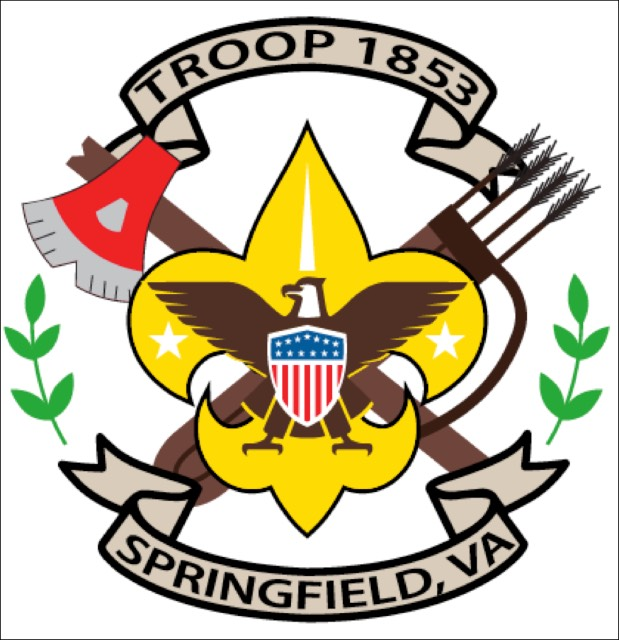
\includegraphics[scale=0.25]{TroopLogo.jpg}}
	\hfill
	\subfigure{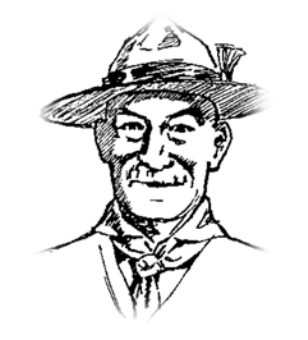
\includegraphics[scale=0.5]{OldMan.jpeg}}
    \vfill
    %\vfill
	\end{figure}
	March 1, 2023
	%\today
\end{titlepage}
\pagenumbering{gobble}
\newpage

\section*{Preface}
The Troop 1853 Handbook is designed to describe in detail what Troop 1853 does and how it operates within the guidelines and regulations of the Chartered Organization and the \ac{BSA}. This handbook is approved by the Troop committee and is applicable to both the \ac{BT} and the \ac{GT}.

This handbook is intended to work with other \ac{BSA} and Troop 1853 policies and is found by the links provided within in the document or on the troop's websites: 

For \ac{BT}: \url{https://springfield1853.mytroop.us} or \url{https://www.troop1853.org}

For \ac{GT}: \url{https://troopwebhost.org/Troop1853SPRINGFIELD} or \url{www.troop1853.com}

This handbook is meant to help guide the actions and activities of Troop 1853. Nothing is intended to add to requirements established by the \ac{BSA}, the \ac{NCAC}, and the \ac{ODD}.

The Troop Committee is responsible for changes and approval of this handbook. Any registered member of Troop 1853 may propose a change to any part of this document, by presenting the change to the Troop Committee at their monthly committee meeting.

\newpage
\section*{Dear Parents, Scouters, and Scouts of Troop 1853,}

This handbook provides information, which will assist you in getting the most out of your Scouting experience - whether you are a parent, Scouter, or Scout. The handbook outlines our policies and describes how we build and implement our program. This is a living document, and it is updated as rules and procedures evolve. It is intended as a supplement to the current \ac{BSA} rules, regulations, and publications. It explains how Troop 1853 operates and is applicable to both the \ac{BT} and the \ac{GT}.
 
The handbook is available on the troop website:
\url{https://springfield1853.mytroop.us//} or \url{https://www.troop1853.org} for the \ac{BT} and \url{https://troopwebhost.org/Troop1853SPRINGFIELD/} or \url{www.troop1853.com} for the \ac{GT}. 

If you have any questions, which are not covered in this handbook, please let me or one of the \acp{SM} know. We have a host of Scouters who can help find the answer.

Remember, none of the Scouter positions in the troop - The Committee, \ac{SM}, \acp{ASM}, or Patrol Advisors -- is gender-specific! We invite both mom and dad to help us!

We will include the resolution of any issues in the next update to the handbook. Please send any recommended changes to the Committee Chair. Our sole purpose is to support our Scouts and provide the best Scouting program possible. We are always interested in additional adult assistance. Please make some time to help out, we can always use your help to improve the troop and the Scouting experience. This is YOUR troop. Help us, Help you, by Delivering the Promise of Scouting to OUR Scouts.



Yours in Scouting,\\ 
Richard C Wink\\ 
Committee Chairman\\ 
1 March 2023

\newpage
\tableofcontents

\newpage

\pagenumbering{arabic}

\section{TROOP 1853 OVERVIEW AND ORGANIZATION}

\subsection{TROOP 1853 HISTORY AND OVERVIEW}
Boys Troop 1853 was chartered in 1969 and Girls Troop 1853 was chartered in 2019. Our goal is to help achieve the mission of Scouting: “To prepare young people to make ethical and moral choices over their lifetimes by instilling in them the values of the Scout Oath and Law.” This includes providing all Scouts the opportunity to earn the rank of Eagle Scout through the implementation of the Aims and Methods of Scouting. Together, \ac{BT} and \ac{GT} have directly affected the lives of several hundred, if not several thousands of youth living in the West Springfield area. We strive hard to have a Scout-led troop.

\subsubsection{TROOP 1853 WEEKLY MEETINGS}
Troop 1853 meets weekly on Tuesday nights from 7:30 PM to 9:00 PM at the Community Covenant Church, unless otherwise announced in advance (e.g., Swimming pool night, special program locations, summer camp week, etc). The troop calendars have meeting locations and times. Exceptions to this are discussed in section \ref{TROOP MEETINGS}.

\subsubsection{TROOP 1853 MONTHLY CAMPOUTS AND SUMMER CAMP}
The troop outdoor program includes a monthly weekend campout (Friday night to around noon Sunday). The Scouts select these monthly activities during the annual planning conference. Each summer, usually in July, the troop attends a one-week summer camp. This camp is especially important for new Scouts and provides an excellent opportunity to work on basic rank requirements and merit badges; it also provides opportunities for older Scouts to try new merit badges or activities.

\subsection{DISTRICT AND COUNCIL}
Troop 1853 is part of the \ac{ODD} and the \ac{NCAC}. We participate in camporees with the \ac{ODD} and occasionally with other Scouting organizations, such as the West Point Camporee, other Districts, and \ac{NCAC}. This is planned by the Scouts during the annual planning conference.

\subsection{TROOP 1853 CHARTERED ORGANIZATION AND REPRESENTATIVE}
The \ac{BSA} does not operate Scout troops. The \ac{BSA} charters organizations to use the program as a resource for youth and families. Because the program of the \ac{BSA} is conducted only through chartered organizations, it is imperative that these  receive effective and meaningful support. Our Chartered Organization is the Community Covenant Church at 7018 Sydenstricker Road, Springfield, VA 22152. The \ac{COR} is selected by the Chartered Organization. Contact with the \ac{COR} is normally through the Troop Committee Chair. The Community Covenant Church Pastor(s) are the Institutional Head and they appoint the \ac{COR}. In some circumstances the Church Committee Chair can/will serve as the institutional Head. The \ac{COR} Guidebook (511-42116) from the \ac{BSA} is a further resource on the roles of the Chartered Organization.

\subsection{TROOP 1853 ORGANIZATIONAL STRUCTURE}
The \ac{BT} and \ac{GT} follow the standard \ac{BSA} Troop organizational structure. This may be modified as practical to meet the needs of the organization by the Troop Committee.

\subsubsection{TROOP RESPONSIBILITY, POSITIONS, FUNCTIONS AND PROCESSES}
\paragraph{TROOP COMMITTEE}
\subparagraph{RESPONSIBILITY}
The Committee's primary responsibility is to support both the \ac{BT} and \ac{GT} leadership in delivering a quality program. These responsibilities include setting policy, helping the troop leadership with the outdoor program and other planned activities, staffing key functions such as advancement and registration, and ensuring financial support. If needed, the Committee acts as arbiter between the \ac{GT} and \ac{BT} \acp{SM}. The committee is also responsible for convening \acp{BoR}  for the advancement of Scouts. More information on \acp{BoR} is found in section 7.5. %ref

\subparagraph{POSITIONS}
The following are key committee positions the troop desires filled at all times to allow proper support to the troop's Scouting program. The Troop 1853 Scouter Position Guide lists additional committee positions, their job descriptions and essential job functions.

\begin{itemize}
	\item \ac{COR} - The \ac{COR} is the direct contact between the committee and the Chartered Organization. The Chartered Organization appoints the unit committee chair and \acp{SM}.

	\item Troop Committee Chair - The troop committee chair is appointed by the chartered organization to see that all committee functions are carried out. The troop committee chair appoints and supervises the unit committee and unit leaders, and organizes the committee to see that all committee responsibilities are delegated, coordinated and completed. There is only one Troop Committee Chair.

	\item Troop Treasurer - The Troop Treasurer is appointed by the committee chair to handle troop funds, pay bills, maintain accounts, and create the yearly budget. The Troop Treasurer will oversee the escrow program, escrow coordinator and troop fundraising activities. The Troop Committee Chair may appoint a \ac{BT} and \ac{GT} Troop Treasurer.

	\item Troop Advancement Chair - The unit advancement chair is appointed by the committee chair to ensure both the \ac{BT} and \ac{GT} have at least monthly \acp{BoR}, periodic \acp{CoH}, and have goals of helping each Scout advance in rank. They support the troop goal by informing the \ac{SM} of new Scouts to reach First Class rank during their first year. The advancement chair is also responsible for record keeping and submitting advancement reports. The Troop Committee Chair may appoint a \ac{BT} and \ac{GT} Troop Advancement Chair.

	\item Troop Membership Chair - The troop membership chair is appointed by the committee chair to ensure that the unit is chartered annually and to ensure that new youth and adult applications along with funds are completed and turned in to the committee chair for processing. The membership chair will support the troop's recharter, recruitment, and retention functions. The Troop Committee Chair may appoint a \ac{BT} and \ac{GT} Troop Membership Chair.

	\item Troop \ac{BoR} Chair- Serves as the focal point for Scouts to request \acp{BoR}. Other tasks include : Collects the required documentation; publishes dates for \acp{BoR}; solicits \ac{BoR} members; briefs members on their duties; ensures acp{BoR} are held according to \ac{BSA} rules and according to Troop 1853 standards; provide feedback on advancement progress and \ac{BoR} comments from the youth to the committee/\ac{SM}.

	\item Scoutmaster - The \ac{SM} of the \ac{BT} and \ac{GT} is nominated by the committee to the Charter Organization who will make the formal appointment. As a member of the committee, the \acp{SM} are responsible for briefing the activities, advancement, service, and other aspects of Scouting for the respective \ac{BT} and \ac{GT}.

	\item Charter Organization - The charter organization, in our case, the Community Covenant Church, annually agrees to the following responsibilities:
	\begin{enumerate}
		\item Appoint the Troop Committee Chair, \ac{BT} and \ac{GT} \acp{SM}, and First and Second \acp{ASM}.
		\item Provides a meeting place and promotes a good Scouting program.
		\item Conduct the Scouting program consistent with \ac{BSA} rules, regulations, and policies.
		\item Approve adult membership applications.
	\end{enumerate}
\end{itemize}

\subparagraph{FUNCTIONS}
The Troop Committee has several positions and a number of functional areas. At times some of these positions may be filled by \acp{ASM}, but the goal is to create active committee members who supports both the \ac{BT} and \ac{GT} at the committee level. These functions include:

\begin{itemize}
	\item Ensures quality adult leadership. Additionally, ensures that all adult leadership is approved, registered, trained and current in \ac{YPT} and position specific training.

	\item Selects and nominates the \ac{SM}, the First \ac{ASM}, and Second \ac{ASM} to the Charter Organization. In case those positions are unfilled, absent for an extended period of time, or an individual is unable to serve, a qualified \ac{ASM} is appointed until the committee can recruit a replacement.

	\item Ensures troop activities are following the \ac{BSA} Guide to Safe Scouting (\url{https://www.scouting.org/health-and-safety/gss/}) and Youth Protection guidelines (\url{https://www.scouting.org/health-and-safety/gss/gss01/}).

	\item Advises the \acp{SM} on policies relating to Scouting and the chartered organization.

	\item Is responsible for finances to include ensuring adequate funds and disbursements are in line with the approved budget plan.

	\item Obtains, maintains, and properly cares for troop property.

	\item Ensures the troop has a quality program that includes an outdoor program (minimum ten days and nights per year). This is reviewed and approved annually.

	\item Ensures members serve on \acp{BoR} and support \acp{CoH}.

	\item Supports the \acp{SM} in working with individual youth and problems that may affect the overall troop program.

	\item Provides for the special needs and assistance some youth may require.

	\item Assists the \acp{SM} with handling youth behavioral problems.
\end{itemize}
The Troop Handbook is updated and approved at a minimum of every five years or sooner at the discretion of the Committee. The Troop 1853 Handbook is approved by the Committee.

\subparagraph{PROCESS}
The committee meets once a month, usually the first Monday of the month. Any Scout or Scouter registered with the \ac{BT} or \ac{GT} may attend. Any parent or guardian with a Scout registered in the \ac{BT} or \ac{GT} is encouraged to attend. Voting members of the committee are those adults registered with either troop in a committee member status. A Scouter fulfilling a Troop 1853 committee responsibility but registered as an \ac{ASM} or another position within the troop are welcome and encouraged to attend but are not voting members. All \ac{BT} and \ac{GT} meetings are open to any parent or guardian of a registered \ac{BT} or \ac{GT} Scout and any registered Scouters of \ac{BT} or \ac{GT}.

\subparagraph{UNPUBLISHED AD HOC POLICIES}
From time to time, both the Scout and adult leaders of the \ac{BT} or \ac{GT} may establish temporary policies that are not reflected in this handbook. It is the responsibility of the policy sponsor to promptly bring these policies to the attention of the Troop Committee for its  ratification, amendment, or termination.

\paragraph{\ac{SM} AND \ac{ASM} POSITIONS, RESPONSIBILITIES, AND FUNCTIONS}
\subparagraph{SCOUTMASTER}
The \ac{SM} provides leadership to the youth through the \ac{PLC} and to the \acp{ASM} by providing guidance and activity coordination. The \ac{SM} serves as the bridge between the \ac{PLC} and the Troop Committee.

\ac{BT} and \ac{GT} has a "First Assistant Scoutmaster" and a “Second Assistant Scoutmaster.” The "First Assistant Scoutmaster," acts in the absence of the \ac{SM}. The “Second Assistant Scoutmaster” acts in the absence of the \ac{SM} and the First Assistant Scoutmaster. Normally the First Assistant Scoutmaster and the Second Assistant Scoutmaster “move-up” when the \ac{SM}'s term is over every two years. The new \ac{SM} then selects a new "Second Assistant Scoutmaster" who must be nominated by the committee to the Charter Organization, who makes the final appointment.

\subparagraph{ASSISTANT SCOUTMASTERS}
The \ac{SM} designates \acp{ASM} who serve in the advisor role for select positions. These could include, but are not limited to the Patrol Advisor, Venture Program Coordinator, Troop Instructor Advisor, and the \ac{OA} Advisor. Additional \acp{ASM} may be designated to assist with functions such as New Scout Training, \ac{ILST}, and Religious Awards.

An \ac{ASM}, Scouter, Parent or Guardian is assigned to each outdoor event and is responsible for the planning      and implementation of the event based on objectives established by the \ac{PLC}. This \ac{ASM}, Scouter, or Parent is designated the \ac{SMIC} and is assisted by other adults and the \ac{SPL} and or a senior Scout designated by the \ac{SM}. The Annual Planning Conference and \ac{PLC}s will assist the \ac{SMIC} and \ac{SPL} in refining the outdoor event. The \ac{BT} and \ac{GT} website has resources to assist the \ac{SMIC} in the execution of their duties.

The \acp{SM} and the \acp{ASM} have the responsibility of working with the youth as they advance along the Trail to Eagle. All Scouters, Parents and Guardians, and Scouts have responsibility in facilitating execution of the troop program.

\Acp{ASM} may be assigned specific duties by the \acp{SM} to assist the Troop Committee.

\Acp{ASM}, being the Adults with the most direct contact with the Scouts, are expected to obtain and wear a complete Scout Uniform and set the standard for uniform wear.

\subparagraph{ASSISTANT SCOUTMASTERS - PATROL ADVISORS}
\begin{itemize}
	\item The \ac{SM} will assign one or more \acp{ASM} to each patrol as Patrol Advisors.
	\item They advise the \ac{PL} on the operation of the patrol; they do not lead the patrol.
	\item Patrol Advisors ensure that training on Scout skills, leadership and outdoorsmanship is conducted properly, and guide the \ac{PL} with training and advancement as required. The Patrol Advisor works through the \ac{PL} on Patrol activities, advancement, and responsibilities (troop program, opening and closing ceremonies, outings, \acp{CoH}, etc.).
	\item The Patrol Advisors guide the employment of Troop Guides in support of the \ac{PL} and patrol activities, provide periodic input on their performance, and recommend to the \ac{SM} whether or not they should receive leadership credit for their term.
	\item Teaching, coaching, mentoring, and evaluation of Scout Spirit are critical functions of a Patrol Advisor. The Scout Spirit rank requirement, from Scout to First Class rank, should be signed off by the Patrol Advisor prior to the Scout completing the \ac{SM} Conference.
\end{itemize}

\subparagraph{ASSISTANT SCOUTMASTERS - POSITION ADVISORS}
\begin{itemize}
	\item \acp{ASM} are assigned by the \ac{SM} to each of the troop officers who performs a specialized function (\ac{OA} Representative, Scribe, Quartermaster, Librarian, Historian, Bugler, Outdoor Ethics Guide, and Chaplain Aide). The \ac{SM} will assign the \ac{ASM} to be a Position Advisor. Note: An \ac{ASM} may have more than one advisory role.
	\item These advisors are responsible to assist Scouts with their assigned Scout position as listed in the Troop 1853 Scout Leadership, Positions of Responsibility, and Election Process Guide.
	\item Position advisors monitor the performance of the Scout, provide coaching and instruction as required, and periodically counsel the Scout on their progress.
	\item At the conclusion of the Scout's term, the position advisor recommends to the \ac{SM} whether or not the Scout successfully met the standards of their job.
\end{itemize}

\subparagraph{EAGLE COORDINATOR / MENTOR / COACH}
On reaching the Life rank, each Scout in either troop is assigned a Troop 1853 Eagle Coach to assist them in navigating the steps to the rank of Eagle Scout. The Eagle Coach is a resource and mentor through the Eagle process. The \ac{NCAC} provides an Eagle Scout Procedures Guide, which can be found at: \url{https://www.ncacbsa.org/eagle-scout-information/}.

\subparagraph{PATROL LEADERS' COUNCIL} 
The \ac{PLC}, not the adult leaders, is responsible for planning and conducting the troop's activities. The \acp{SM} with support from the \acp{ASM} provide direction, coaching, and training that empower the \ac{PLC} members with the skills they will need to lead the troop. The Troop Committee provides resources to help the \ac{PLC}.

The \ac{PLC} constitutes the Scout leadership for Troop 1853. There are separate \acp{PLC} for both the \ac{BT} and \ac{GT}. The \ac{SPL}, \acp{ASPL}, the \acp{PL}, Troop Guides, Troop Instructors, and the Troop Officers (Quartermaster; Chaplain Aide; Historian; Librarian; Bugler, \ac{TOAR}, Outdoor Ethics Guide, and Scribe) comprise the \ac{PLC}. See Section 1.4 (ADD REFERENCE) Troop Organizational Structure for a graphical and hierarchical depiction. While all Scouts may attend the \ac{PLC}, those listed above are required to attend or be excused by the \ac{SM}.

The Troop 1853 Scout Leadership, Position of Responsibility, and Troop Election
Process Guide (available on the websites) provides detailed information on Troop Leadership Position Information and Eligibility Requirements to include roles and responsibilities. It highlights the training and attendance requirements for each leadership position. The Troop 1853 Election process is explained in the Troop Election Process Guide. The Troop 1853 Scout Leadership, Position of Responsibility, and Troop Election Process Guide is on the troop website under references.

The \ac{PLC} plans the yearly troop program at the annual planning conference,  usually held in June. The \ac{PLC} meets monthly to develop plans for upcoming meetings and activities. All troop leadership is expected to attend both the annual planning conference and the monthly \ac{PLC} meetings in order to receive leadership credit.

\subparagraph{GREEN BAR}
Green Bar History. The Green Bar is named for William “Green Bar Bill” Hillcourt. Mr. Hillcourt wrote many of the best resources for Scouts and Scouters starting with handbooks for \acp{SM} and \acp{PL} in the 1920's. Green Bar Leadership Positions historically are based upon the Scout Leadership patches containing a “green bar” and are the \ac{SPL}, Troop Guides, \acp{PL}, and \ac{APL}s.

In Troop 1853, we consider the \ac{SPL}, \acp{ASPL} and in certain situations, the Senior Scout a Green Bar. The \ac{JASM} is included when the \ac{SM}, in coordination with the Troop Committee, appoints a \ac{JASM}. The \ac{SPL} and \acp{ASPL} are not assigned to a Patrol as they are considered troop level leadership.

On campouts and other troop events, Troop 1853 Green Bar may eat and share camp responsibilities with the adult's Patrol. Troop Guides, \acp{PL} and \ac{APL}s will eat and camp with their assigned patrol.

\subparagraph{PIRATES PATROL}
The activation and deactivation of the Pirates Patrol or other 'senior Scout' patrol is at the discretion of the \ac{SM} in consultation with the Committee Chairman.
Historically a \ac{BT} patrol, the Pirates Patrol provides Scouts in the troop who have served in specific leadership positions within Troop 1853 an opportunity to build and operate their own program. To belong to the Pirates Patrol is a privilege, not a right. The Pirates Patrol member must meet eligibility listed below and receive approval of the \ac{SM}. The \ac{SM} may add or remove a Scout assigned to the Pirates Patrol. 

The Pirates Patrol program, while remaining tied into the overall troop program, allows the patrol members to participate in activities and programs that are more challenging and meaningful to their needs and interests. The Pirates Patrol will support the patrol and troop programs and lend their experience with the intent to improve overall program success.

\textit{Standards}
\begin{itemize}
	\item As a minimum, the Pirates Patrol will adhere to the same standards and rules as the regular patrols and will actively participate, as defined by the SM, in the troop program. They may be assigned a specific program month by the \ac{PLC}.
	\item Troop 1853 expects that due to their previous leadership experience and rank they will exceed these standards and serve as role models for all other Scouts in the troop.
	\item On selected occasions, special privileges may be afforded to the Pirates as determined by the \ac{SPL}, \ac{SM}, or \ac{SMIC}, as appropriate, in keeping with the special trust afforded based upon their previous service and leadership to the troop.
\end{itemize}

\textit{Eligibility}
\begin{itemize}
	\item Scouts will be eligible to join the Pirates Patrol if they:
	\begin{itemize}
		\item have successfully served as a \ac{PL}, \textit{and} as either \ac{SPL} or \ac{ASPL}
		\item are not currently serving as PL of another patrol, \ac{SPL} or \ac{ASPL}
		\item are at least Life Rank
		\item receive approval of the \ac{SM}
	\end{itemize}
	\item The \ac{SM} may allow other Scouts not meeting the requirements above to join the patrol when there are special circumstances.
	\item Members of the Pirates Patrol who desire to serve as Troop Guide, Instructor, or Den Chief will be encouraged to do so. They will be expected to fulfill all of their responsibilities in these positions.
\end{itemize}

\textit{Program}
\begin{itemize}
	\item The Pirates Patrol's program will be built on service and support to Troop 1853.
	\item The Pirates Patrol may have periodic patrol activities.
\end{itemize}

\textit{Camping:} 
The Pirates Patrol will have their own patrol equipment and will participate in campouts as their own patrol, cooking their own meals and setting up their own campsite. Pirates may tent individually and use hammocks from April to October. At the discretion of the SMIC, based upon campout program considerations and in coordination with the \ac{SM} they may merge with the adult's Patrol for the campout.

\textit{Participation:}
The Pirates Patrol is a troop-level asset that the \ac{SPL}, \acp{ASPL}, \acp{PL}, Patrol Advisors, SMIC, the \ac{SM} and others within the troop leverage to assist in the planning and execution of other programs, activities and advancements. Pirate Patrol members may fill in as a de facto Troop Instructor.

Pirates Patrol members will direct and assist with troop activities. These examples include:
\begin{itemize}
	\item Assisting the \ac{PLC} to lead ILST.
	\item Assisting with new and newly assigned Scouts.
	\item Overseeing Tenderfoot physical fitness tests.
	\item Assisting with training for Fireman Chit and Tot'n Chip.
	\item Assisting with summer camp preparation.
	\item Teaching Scout Skills on campouts, summer camp, and other troop events.
\end{itemize}

The Pirates Patrol will not participate in the Troop Honor Patrol competition. However, they are expected to set the example for the other Patrols and to assist their assigned Patrol if they are a Troop Guide. They may participate in earning the recognition of a \ac{NHP}.

\subsubsection{ADDING/REMOVING PATROLS}
The size of the troops continually grows and shrinks. At the discretion of the SM, in consultation with the Committee Chairman, they will adjust the number of patrols to accommodate this fluctuation. Optimally, patrol size should be 8-10 active Scouts. This allows for a sufficient number of Scouts for the \ac{PL} to guide, without placing an excessive burden on them. This size for patrols also allows for adequate opportunities for leadership positions. The \ac{SM} will determine who meets the “active” criteria. Generally, it includes frequent participation in meetings, activities and campouts.

\section{TROOP GUIDEPOSTS}
\subsection{GUIDING PRINCIPLES}
The guiding principles of Troop 1853 are the \ac{BSA} Mission, Aims and Methods of Scouting. The Troop 1853 goal is to maximize opportunities for Scouts to experience the Scouting values while having fun.

\subsubsection{SAFETY}
Safety is a vital concern to the troop and all safety regulations and policies established by the \ac{BSA} and the Chartered Organization will be enforced. During all activities, Troop 1853 will follow \ac{BSA}'s Guide to Safe Scouting, which can be found at:  \url{https://www.scouting.org/health-and-safety/gss/}  Scouts who repeatedly violate safety rules may be sent home from the activity. Safety is everyone's responsibility.

\subsection{MISSION}
The mission of the \ac{BSA} is to prepare young people to make ethical choices over their lifetime by instilling in them the values of the Scout Oath and Law.

\subsection{AIMS}
The Scouting program has specific objectives, commonly referred to as the “Aims of Scouting.” They are \textbf{character development, leadership development, citizenship training, and personal fitness}. Leadership development is also one of Scouting's eight methods contributing to both good character and good citizenship.

\subsection{METHODS}
The methods by which the Aims are achieved are listed below in random order to emphasize the equal importance of each.

\subsubsection{IDEALS}
The ideals of Scouting are spelled out in the Scout Oath, the Scout Law, the Scout motto, and the Scout slogan. The Scout measures themselves against these ideals and continually tries to improve. The goals are high, and, as they reach for them, they have some control over what and who they become.

\subsubsection{PATROLS}
The patrol method gives Scouts an experience in group living and participating citizenship. It places responsibility on young shoulders and teaches Scouts how to accept it. The patrol method allows Scouts to interact in small groups where they can easily relate to each other. These small groups determine troop activities through their elected representatives.

\subsubsection{OUTDOOR PROGRAMS}
Scouting is designed to take place outdoors. It is in the outdoor setting that Scouts share responsibilities and learn to live with one another. It is here that the skills and activities practiced at troop meetings come alive with purpose. Being close to nature helps Scouts gain an appreciation for God.

\subsubsection{ADVANCEMENT}
Scouting provides a series of surmountable obstacles and steps in overcoming them through the advancement method. The Scout plans their advancement and progresses at their own pace as they meet each challenge. The Scout is rewarded for each achievement, which helps them gain self-confidence. The steps in the advancement system help a Scout grow in self-reliance and in the ability to help others.

\subsubsection{ASSOCIATION WITH ADULTS}
Scouts learn a great deal by watching how adults conduct themselves. Scout leaders can be positive role models for the members of their troops. In many cases a \ac{SM} who is willing to listen to the Scouts, encourage them, and take a sincere interest in them can make a profound difference in their lives.

\subsubsection{PERSONAL GROWTH}
As Scouts plan their activities and progress toward their goals, they experience personal growth. The Good Turn concept is a major part of the personal growth method of Scouting. Young people grow as they participate in community service projects and do Good Turns for others. Probably no device is so successful in developing a basis for personal growth as the daily Good Turn. The religious emblems program also is a large part of the personal growth method. Frequent personal conferences with their \ac{SM} help each Scout to determine their growth toward Scouting.

\subsubsection{LEADERSHIP DEVELOPMENT}
The Scouting program encourages Scouts to learn and practice leadership skills. Every Scout has the opportunity to participate in both shared and total leadership situations. Understanding the concepts of leadership and becoming a servant leader helps a Scout accept the leadership role of others and guides them towards participating citizenship and character development.

\subsubsection{UNIFORM}
The uniform makes the Scout troop visible as a force for good and creates a positive youth image in the community. Scouting is an action program, and wearing the uniform is an action that shows each Scout for Scout activities and provides a way for Scouts to wear the badges that show what they have accomplished. Scouts and \acp{ASM} are expected to make every effort possible to wear the correct uniform for each function. Leadership will make every effort to publish and inform everyone of any changes. 

\paragraph{THE TROOP 1853 - \ac{BSA} UNIFORM}
Normally any Scouting event associated with Troop 1853 will require either the Field Uniform or the Activity Uniform. A good rule of thumb is to wear the Activity Uniform shirt under the Field Uniform shirt, that way the Scout has both uniforms just in case. The troop will make accommodations to help Scouts obtain uniform pieces if they need assistance and have a demonstrated need. We have a uniform locker in the basement in which to donate or purchase uniforms items. Each uniform item is \$5, paid to the Troop Treasurer or Troop Uniform Coordinator. The T-Shirt coordinator can also order you additional Troop 1853 activity shirts (long or short sleeve), fleeces, and hats. Troop 1853 believes that a full uniform is an important part of the program and expects Scouts to obtain and wear one.

\subparagraph{FIELD UNIFORM (unofficially known as the “Class A” Uniform)}
Scouts wear the field uniform to troop meetings and traveling to/from all Scouting events, including campouts. The Activity Uniform may be worn to troop meetings during the summer months, but this will be announced ahead of time. The Field Uniform is mandatory all year long for the \ac{SM} Conference, \ac{BoR}, and \acp{CoH}. The full Field Uniform is listed below. In Troop 1853 Scout lingo, 'being full' means you are wearing all of the uniform pieces. After the start of each troop meeting, the \ac{PL} will report the number of patrol members present and if they are in full uniform. If it comes down to attending the meeting not in uniform or not attending the meeting at all, we want your Scout to attend the meeting.

Field Uniform
\begin{itemize}
	\item \ac{BSA} official long- or short-sleeve tan Shirt with green shoulder loops on epaulets
	\item \ac{BSA} Troop 1853 Neckerchief (supplied by the troop), other Scout-related neckerchief, or Scout related Bolo Tie
	\item \ac{BSA} official olive-colored Pants or Shorts; no cuffs or olive Skort for the \ac{GT} (at the discretion of the SMs, olive colored Pants or Shorts may be substituted for the official \ac{BSA} items)
	\item \ac{BSA} official Socks or hiking socks if wearing hiking boots
	\item Official Scout web Belt with \ac{BSA} insignia on buckle, or official leather belt with buckle of your choice or \ac{BSA} official pants or Shorts with sewn in belt.
	\item Hiking Boots or other appropriate footwear (i.e. close-toed shoes). Hiking boots are mandatory on campouts.
\end{itemize}

\subparagraph{ACTIVITY UNIFORM (unofficially known as the “Class B” Uniform)}
This is worn for daily routines during Scout functions, during campouts, Scouting activities, summer time, and any “work” type of Scout activity. The activity uniform is a fill-in uniform for when the field uniform is not appropriate. The \ac{PL} or \ac{SPL} will decide if these are required for a particular meeting or event, or if any other type of shirt or item will be permitted.

Activity Uniform
\begin{itemize}
	\item \ac{BSA} Troop 1853 T-shirt or other Scout related T-shirt
	\item \ac{BSA} official olive-colored Pants or Shorts; no cuffs, or olive Skort for the \ac{GT} (at the discretion of the SMs, olive colored Pants or Shorts may be substituted for the official \ac{BSA} items)
	\item \ac{BSA} official Socks or hiking socks if wearing hiking boots
	\item Official Scout web Belt with \ac{BSA} insignia on buckle, or official leather belt with buckle of your choice or \ac{BSA} official pants or Shorts with sewn in belt.
	\item Hiking Boots or other appropriate footwear (i.e. close-toed shoes)
\end{itemize}

\subparagraph{OTHER}
\begin{itemize}
	\item Sandals, flip-flops, or open-toed shoes MAY NOT be worn with any uniform or on campouts. Some activity areas (swimming pools, bath houses, etc.) may require an exception to this rule; such an exception will be announced in advanced by the \ac{SM} (Note- the expectation is that Adults participating or attending these functions set a proper example as well)
	\item Hats and jackets are acceptable and encouraged for outdoor activities. Hats are generally NOT worn indoors - especially at the church. The weather will usually determine the best type of hat to wear (i.e. brimmed or stocking cap). Scout-inappropriate logos will not be worn.
\end{itemize}

\subparagraph{\ac{BSA} UNIFORM SHEET}
The \ac{BSA} Uniform inspection sheet can be found at on the troop websites. This provides further details on patch  locations and other uniform items. It can also be found in the Scout Handbook.

\subsection{SCOUT SPIRIT}
What is Scout Spirit? - The way in which a Scout demonstrates their commitment to Scouting is through living by the Scout Oath and Law. Doing a daily Good Turn is one of the best ways in which a Scout can show their Scout Spirit. Scouts also demonstrate Scout Spirit when they participate in service projects of the troop, when they help the troop with troop and patrol events and activities, and by providing service to their school, their respective churches, mosques, synagogues, and their community as a whole.

\subsection{STANDARD OF CONDUCT}
All Scouts, Scouters, Merit Badge Counselors, parents, and friends are expected to live by the Scout Oath and Law. This must be followed both in daily conduct, and in the resolution of any disagreements. Behavior and discipline are discussed further in Chapter 10 Troop 1853 Rules of Behavior and Discipline Policy / Procedures (ADD REFERENCE).

\subsection{DISPUTE RESOLUTION}
In every organization, there are disputes; they are inevitable and should be dealt with as quickly as possible.

The first alternative is to talk over the dispute with the individual(s) involved.
Scouts should try to resolve their own problems rather than the parents -- its part of the training program. If the Scouts cannot resolve the problem themselves, they should then go to their \ac{PL}, the \ac{SPL}, and then the \ac{SM} (or Patrol Advisor) if the situation is not resolved.

Parents should discuss their concerns with the patrol advisors and if not resolved, should discuss them with the \ac{SM}. Scouters should talk first to the individuals involved, then the \ac{SM}. If the dispute is not resolved, then the parent should present the issue to the Troop Committee for resolution.

\subsection{ACTIVITIES AND ITEMS NOT ALLOWED}
The troop does not permit Scouts to use sheath knives or folding knives with blades over 3 1/2 inches long. Scouts must earn the Tot'n Chip to use and carry a knife. Scouts must exercise extreme care in properly storing their folding knife at home. For example, Scouts should use care when using their day pack for both school and Scout activities so they don't accidently bring a knife to school. Scouts may only bring two knives, including a multi tool type tool, to weekend and camp activities.

Use of entertainment devices are only allowed in vehicles when traveling to and from a troop activity. They may not be brought into camp even if they are not used there. Scouts will not have firearms or any items which are otherwise illegal such as fireworks, vaping  devices, cigarettes, or drug paraphernalia. Inappropriate reading or pornographic material is  also not allowed.

Under no circumstances is anything which contains a flame allowed in tents, shelters, or other prepared structures.

Scouts are forbidden from departing the activity area without the express permission of one of the adult leaders. Sign-out sheets will be maintained by the SMIC to account for those Scouts leaving and returning from other activities (sports games and school events for example). Departures must be coordinated in advance and the adult picking up the scout should be authorized to do so by a legal guardian of the Scout.

\subsection{TROOP 1853 TECHNOLOGY POLICY}
\subsubsection{GENERAL GUIDELINES}

\begin{itemize}
	\item Use the technology to build relationships with the troop, find useful information, communicate, and share excitement about Scouting.
	\item Updates to social sites using appropriate, (non-embarrassing), photos or clips can share and build excitement about Scouting.
	\item Don't let technology detract from the outdoor experience, the program experience, or the Scouting experience for the troop or patrol.
	\item Teach Technology use. We don't ban acceptable knives, hand axes or gas lanterns; we teach their use. Similarly, we don't ban technology. We teach its use.
\end{itemize}

\subsubsection{GENERAL USE}
Troop 1853 supports the use of technology as a useful tool. The Scout Law should guide the use of technology devices. The device should not be a distraction. Scouts should pay attention to the program and fellow Scouts. In a program or troop situation, a Scout should avoid checking their device for incoming messages or postings. Scouts should not become overly reliant on the device. For example, a Scout should be ready with their map and compass rather than rely on a device's GPS.

\subsubsection{TECHNOLOGY RESPONSIBILITY}
The care, use, security, cost, and power requirements of the technology device is the responsibility of the Scout. The Scout is responsible for any and all costs associated with the use of the technology device; these may include voice, text, data plans, and application purchases or use. The Scout may request to secure their technology device in a vehicle or lock box during the campout. The Troop will assume no responsibility or liability for the loss or damage of any  device. When in doubt, leave them at home.

\subsubsection{TECHNOLOGY DISCIPLINE AND REPERCUSSIONS}
Should any \ac{PL}, \ac{SPL}, \ac{ASM} / \ac{SM}, determine the technology in use is not in support of the activity or being properly used in accordance with the Scout Law they will request the Scout put away the device until the end of the activity. The \ac{SPL}, \ac{SM}, or \ac{SMIC} may determine that the technology device should be taken away from the Scout for the remainder of the event. If taken away the device will be secured in a vehicle or lock box. If the use of a device continues to be problematic, the \ac{SM} will discuss the issue with the Scout's parent.

\section{TROOP 1853 MEMBERSHIP, RECHARTER, RECRUITMENT AND RETENTION}
\subsection{TROOP RECHARTERING, DUES, REGISTRATION}
Rechartering is conducted by the Troop Membership chair on an annual basis. All troop members will support the annual process by completing training, paying dues, and updating information as requested by the membership chair. Any Scout or Scouter who expects to be registered with Troop 1853 during the annual rechartering must complete \ac{YPT} and pay their dues. Any Scouter who is not current in their \ac{YPT} may not reregister. All Scouters should work to become fully trained in their role. 

\subsubsection{ANNUAL DUES AND FEES}
Dues and Fees are reviewed and set each year by the Unit Committee. This is normally done during the September Committee meeting. The fees portion pays for the annual registration fee to the National Council of \ac{BSA} and \ac{BSA} Insurance. A subscription for Scout Life magazine may be included for an additional fee and is encouraged as a great source of Scouting information. The dues portion covers troop operating/administrative expenses and capital replacement costs. It does not pay for campouts, summer camp, or high adventure activities. Those are self-sustaining. 

Registration fees for Scouters are also established by the unit committee. These include all \ac{BSA} fees and insurance and include a dues portion. Those registering with the \ac{ODD} as Merit Badge Counselors, Nova Counselors and Supernova mentors are not charged an annual registration fee.

\subsection{TROOP RECRUITING}
Troop 1853 actively recruits from Cub Scout Packs in the local area. Historical success has been achieved through an active Webelos Liaison and Recruiter who reaches out to Cubmasters and Webelos Den Leaders early in the Scouting/School year during the Webelos Arrow of Light Year during September through November timeframe. This allows Den Leader to plan for and visit the troop on a timeline that supports their crossover schedule.

Troop 1853 will usually offer two Webelos Days during troop meeting times. They are focused on Webelos visiting the troop and the meeting is designed to showcase the troop, its Scouts, how we conduct Scouting, and to help the Webelos and their parents determine if the troop is a good fit. The Webelos Liaison and Recruiter coordinate with the \ac{SM} and the \ac{PLC} to inform  them of when Arrow of Light Scouts are visiting the troop so the Program can be planned accordingly. The Webelos days are normally planned for October and February. Additionally, Troop 1853 welcomes any potential new or transferring Scouts to visit during any troop meeting.

Webelos Crossover. Den Leaders and or Cubmaster should advise the Webelos Liaison and Recruiter and or the \ac{SM} of the date of their crossover ceremonies. The \ac{SM}, First \ac{ASM}, or the Second \ac{ASM} will attend the crossover ceremony along with the \ac{SPL} or \ac{ASPL} and the \ac{PL} of the new Scout's Patrol to welcome the Webelos crossing over to Troop 1853. Crossing over Webelos will receive a unit neckerchief, slide/woggle. They will also receive information to complete the transfer to the troop.

Once a Scout has registered and paid their dues, they will receive the remainder of their Scout package. This includes a Scout Handbook, current scout epaulets, patrol patch, Troop 1853 Patch and any other items determined by the troop.

\subsection{SCOUT RETENTION}
The \ac{SM} will review the participation of all Scouts periodically. Scouts not participating over the past several months will be identified and the Patrol Advisors will attempt to determine the Scout's intentions. The \ac{SM} will report to the Troop Committee any systemic issues that are identified which may require corrective action by the troop, the first action then being a special \ac{BoR} as outlined in section 8.0.1.3 of the 2017 \ac{BSA} Guide to Advancement.

\section{TROOP 1853 COMMUNICATIONS}
\subsection{OVERVIEW}
The Troop has several means of communications that include E-mail, Phone calls, announcements at troop meetings, the troop website, and the quarterly “The Eagle” newsletter.

Face to Face communication remains the best form of communication especially between the Scout and Scouter. However, the Troop uses email as it primary communication method, and as such, the Troop does not encourage the use of texting, especially when it is between a Scout and an adult Scout leader. Scouts should refrain from texting adult scout leaders and adults scout leaders should refrain from texting Scouts. Should the need arise for a Scout or Scouter to text, they should include another adult on the text to ensure they follow the \ac{BSA} no one-on-one contact rules. 

The troop has established an email that should be included on all adult to scout communications to ensure no one-on-one discussions. This is to protect both the Scout and the Adult. 

Boys Troop: ypt@troop1853.org
Girls Troop: TBD

This address is delivered to several Adult Scouters who monitor these communications according to the principles of the Guide to Safe Scouting and Youth Protection Guidelines. This also includes other phone or computer applications in which a Scouter or adult could contact the Scout directly without knowledge by the parent or other adult. Time sensitive communication should be handled by a phone call.

\subsection{EMAIL}
Information about activities (e.g., event times, dates, locations, uniform, etc.) comes out in emails from Scouts or Scouters in charge of the activity. These emails should be able to answer most questions about an activity. If you are NOT receiving information via email or you  change your email address, please send an email to:

Boys troop: email@troop1853.org
Girls Troop: TBD

Include all the email addresses you want to be added or removed, and they will update the appropriate distribution list. Any Scout's email address will be added to the troop and the Scout's respective Patrol distribution lists with parent or guardian permission.

Scouts will need an email address or regular access to email. The Scout will need to communicate with their Patrol, \ac{SM}, and other adults or Scouts on certain activities and events. Families will need to plan for access. Will the Scout have their own personal email account or will they share a parent's email? The Scout / Parent should regularly check the email for troop and Patrol information. Email is a critical information dissemination method used by the troop. Be prepared for a lot of emails - the troop errs on the side of over communicating. When the Scout is sending emails to adults they should include a parent or can use the Youth Protection email in the troop Contacts section to ensure there is no one-on-one contact

E-mail groups are used for general announcements (e.g., upcoming meetings, campouts, events). The addresses for these groups will not be provided on the troop website and should not be placed in individual address books. This helps maintain the security of the list and in doing so reduces SPAM.

\subsection{PHONE CALLS}
A phone call should be used for time-sensitive announcements or when you need to solve a problem immediately. Phone numbers are listed in the troop directory. When leaving a voicemail message, include your name, patrol, and phone number. The availability and frequency of Directory updates depends on an adult volunteer being available to generate the Directory. 

\subsection{ANNOUNCEMENTS DURING TROOP MEETINGS}
In addition to email, information is also put out at troop meetings at the start and end of meetings. If you are picking up or dropping off your Scout, you should plan to stay for one or both of these information / announcement sessions. Usually, the person in charge of an event is the one making the announcement at the troop meeting. This is a great time to ask questions. If you are making an announcement it should be less than one minute, additional information can be distributed to the Troop via email or flyers.

\subsection{THE TROOP NEWSLETTER}
“The Eagle” is published every quarter to keep Scouts, Scouters and parents informed and up to date on troop activities.

\begin{itemize}
	\item The newsletter is normally emailed to the troop. It is also posted on the troop web site.
	\item Each issue contains a calendar of events for the next few months. Also included are the Patrol duties for the coming month, news of upcoming activities, reports of recent activities, the \ac{SM}'s Minute, and a report from the Troop Committee Chairman. The Eagle editor will solicit articles a few weeks prior to the publication date. 
	\item Many leadership positions require the Scout to publish one or more articles in The Eagle.
\end{itemize}

\subsection{TROOP CALENDAR}
The troop calendars are available:

Boys Troop: \url{https://www.troop1853.org/event/}

Girls Troop: \url{https://troopwebhost.org/Troop1853SPRINGFIELD/}

You can subscribe to the calendar so troop events show up in your calendar app. 

\subsection{TROOP 1853 WEBPAGE}
Boys Troop: \url{https://www.troop1853.org/}

Girls Troop: \url{https://troopwebhost.org/Troop1853SPRINGFIELD/}

are the troop websites maintained by the Troop Committee to provide an always- available source of information about the troops. In addition, copies of forms (Honor Patrol Worksheets, \ac{PLC} Patrol Forms, permission slips and medical exam forms) are usually available for downloading. Only the first names of Scouts will be shown on the troop  websites.

\subsection{SOCIAL MEDIA}
All Social Media within the troop will follow \ac{BSA} Policy Social Media Policy. 
\url{https://scoutingwire.org/marketing-and-membership-hub/social-media/social-media- guidelines/}

\subsubsection{TROOP 1853 FACEBOOK PAGE}
The troop committee is responsible for the Troop 1853 Facebook page. This page will be administered by Troop 1853 registered Scouters in accordance with the \ac{BSA} Social Media Policy and any Chartered Organization policies. Facebook page members and invitees must be registered with the troop or in some way linked to Troop 1853. These may include parents of current Scouts, former Scouts and or their parents, former Scouters, and or district or council Scouters related to Troop 1853.

\subsubsection{TROOP ALUMNI FACEBOOK PAGE}
The troop committee is responsible for the Troop 1853 Alumni Facebook page. This page focuses mainly on past troop activities in an attempt to keep former members of the troop connected with the troop, and serve as a visual repository of the troop's history. All former members are encouraged to post photographs and comment on those posted. The page features an Eagle Scout Roll Call album, and a collection of past Eagle newsletters.

\subsection{TROOP DIRECTORY}
A troop directory may be published in the spring and fall each year after Troop Elections to reflect new leadership positions. The Directory is only published when an adult volunteer is available and willing to put it together. It should include the address, phone number and e-mail address of the Scouts and the adult leaders, and the rank and age of each Scout. Scouts are listed both alphabetically and by patrol. If no Troop Directory is published it is inherent on Troop Scout Leadership to ensure individual patrol information is shared. Scoutbook may also be used to obtain Scout, Scouter, and adult information.

\subsection{TROOP 1853 INDIVIDUAL AND GROUP CONTACTS}
Should you need to contact Troop 1853 the best person is the \ac{SM} at 
scoutmaster@Troop1853.org 
or the Committee Chair at 
committee\_chair@Troop1853.org.

Other persons of note for the \ac{BT} are listed below:

\begin{tabular}{ l l }
	\textbf{Person or Group} & \textbf{Address} \\
	\hline
	Activities Recorder 				& activities\_recorder@troop1853.org \\
	Advancement Chair 					& advancement\_chair@troop1853.org \\
	Everone (Scouts, Parents, Leaders)	& announce@troop1853.org \\
	Assistant Scoutmasters				& asms@troop1853.org \\
	Board of Review Chair				& bor@troop1853.org \\
	Troop Committee						& committee@troop1853.org \\
	Committee Chair						& committee\_chair@troop1853.org \\
	Troop Zelle Account					& deposits@troop1853.org \\
	Dragons Patrol						& dragons@troop1853.org \\
	Eagle Editor						& eagle\_editor@troop1853.org \\
	Email Administrator					& email@troop1853.org \\
	Greenbar Patrol						& greenbar@troop1853.org \\
	New Scout Recruiting				& info@troop1853.org \\
	All registered adult leaders		& leaders@troop1853.org \\
	Medical Form Coordinator			& medical\_forms@troop1853.org \\
	Membership Chair					& membership\_chair@troop1853.org \\
	Active OA Members					& oa@troop1853.org \\
	Scorpion Patrol						& scorpions@troop1853.org \\
	Scoutmaster							& scoutmaster@troop1853.org \\
	Shark Patrol						& sharks@troop1853.org \\
	Adult Training Chair				& training\_chair@troop1853.org \\
	Treasurer							& treasurer@troop1853.org \\
	Unit College Reserve Members		& unitcollegereserves@troop1853.org \\
	Webelos Liaison						& webelos\_liaison@troop1853.org \\
	Website Administrator				& webmaster@troop1853.org \\
	Wolf Patrol							& wolves@troop1853.org \\
	Youth Protection Email Monitors		& ypt@troop1853.org \\
	\hline
\end{tabular}

Other persons of note for the \ac{GT} are listed below:

\begin{tabular}{ l l }
	\hline
	\textbf{Person or Group} & \textbf{Address} \\
	All Adults 						& all\_adults.Troop1853SPRINGFIELD@twh.email \\
	All Scouts 						& scouts.Troop1853SPRINGFIELD@twh.email \\
	All Troop 						& all\_troop.Troop1853SPRINGFIELD@twh.email \\
	Assistant Scoutmasters			& ASMs.Troop1853SPRINGFIELD@twh.email \\
	CCC Leadership 					& cccleadership.Troop1853SPRINGFIELD@twh.email \\
	Committee 						& committee.Troop1853SPRINGFIELD@twh.email \\
	Committee Chair 				& committee.chair.Troop1853SPRINGFIELD@twh.email \\
	Flaming Cacti 					& cacti.Troop1853SPRINGFIELD@twh.email \\
	Info 							& info.Troop1853SPRINGFIELD@twh.email \\
	Night Owls 						& owls.Troop1853SPRINGFIELD@twh.email \\
	Sales 							& sales.Troop1853SPRINGFIELD@twh.email \\
	Scouters 						& scouters.Troop1853SPRINGFIELD@twh.email \\
	Scoutmaster 					& scoutmaster.Troop1853SPRINGFIELD@twh.email \\
	Scouts Only 					& scouts.only.Troop1853SPRINGFIELD@twh.email \\
	Site Admin 						& siteadmin.Troop1853SPRINGFIELD@twh.email \\
	Treasurer 						& treasurer.Troop1853SPRINGFIELD@twh.email \\
	\hline
\end{tabular}


\section{TROOP 1853 MEETINGS AND CEREMONIES}
\label{TROOP MEETINGS}

\subsection{ATTENDANCE}
The Scout program in general and the troop program in particular are good ways in which Scouts can have fun, learn useful skills and grow in many different ways. This is only possible through regular attendance and participation in troop activities. Because we use the patrol method, absences have an adverse impact on the patrol's ability to perform and on the quality of the program for all of the Scouts.

We recognize that other interests and activities have their seasons. However, overall attendance and participation are factors to be considered in advancement through the Scouting program and certification of leadership time.

Scouting is a year-round program. When individual Scouts or Scouters schedule supplemental troop events (such as Eagle Scout projects, service projects, etc.), they should schedule around the mandatory activities of the troop, which are usually listed in the troop calendar. Individual events should be coordinated with the \ac{SM} and Committee Chair well in advance of the activity to avoid conflicts. Troop 1853 activities take priority over individual Scout or Scouter events.

Registration in the troop, by itself, or simply attending troop meetings, does not satisfy the Scout Spirit and participation requirements for advancement. Scouts must remain active in the troop and support patrol activities in order to qualify for advancement.

If a Scout will not be participating for an extended period of time, they must inform the \ac{SM} in advance and provide an explanation along with a commitment on when they will return.

Scouts who have other obligations, like participation in sports, that prevent normal participation in troop activities, must consult with the \ac{SM} prior to the activities so alternative efforts may be considered as substitutes for satisfying the goal of demonstrating Scout Spirit. Alternative projects can include taking responsibility for planning, supporting, or running a troop program, service event, or outdoor activity.

\subsection{TROOP MEETINGS}
Troop 1853 meets weekly on Tuesday nights from 7:30 PM to 9:00 PM at the Community Covenant Church, unless otherwise announced in advance (e.g., Swimming pool night, special program locations, summer camp week, etc). The troop calendar has meeting location and times.

Scouts are encouraged to attend part of a meeting if they are also involved in school or church activities - even if they do not have their uniform.

In the event that inclement weather on the day of a troop meeting or other troop event causes the Fairfax County public schools to close for the day, to dismiss early, or to cancel after-school activities, the \ac{SM} (in conjunction with the SMIC in the case of an outdoor activity) will determine whether to cancel the meeting or activity by 4 PM. The cancellation will be an email message troop wide as soon as that decision is made. The \ac{SPL} will also notify the Green Bar and notify the \acp{PL} who in turn will notify the members of their patrols. If the schools have a delayed arrival due to inclement weather but school is dismissed on time, the presumption shall be that the troop activity will take place as scheduled unless a troop wide e-mail message provides other instructions.

\subsection{PATROL LEADERS COUNCIL MEETINGS}
The \ac{PLC} usually meets the third Monday of each month. 

All troop leadership is required to attend the monthly \ac{PLC} meeting. In the event that the \ac{SPL} or \ac{PL} cannot attend, they are expected to arrange for an assistant to attend in their stead. \acp{ASM}, Committee  Members, as well as parents are invited to attend the \ac{PLC} meeting. There are multiple Scout leadership positions that have participation in the monthly \acp{PLC} as a condition of receiving full leadership term credit.

The \ac{PLC} purpose is to plan the troop meetings and outdoor activities for the upcoming two to three months based upon the approved troop annual plan determined during the annual planning conference and approved by the troop committee.

The \ac{PLC} meeting begins at 7:30 PM and usually ends around 8:30 PM.

The \ac{SPL} leads the meeting. The \ac{SM}, First and Second \acp{ASM}, Patrol Advisors, the \acp{JASM}, and the \ac{SMIC} for upcoming activities attend these meetings. The \ac{SM} serves as the primary advisor to the \ac{PLC}.

\subsection{ASSISTANT SCOUTMASTER MEETING}
The \ac{SM} meets with the \acp{ASM} once a month, usually immediately after the \ac{PLC} meeting with the intent to determine how best to support the \ac{PLC} in executing the troop program. The \acp{ASM} may meet at a different time to discuss specific issues and long range plans.

\subsection{TROOP COMMITEE MEETING}
The Troop Committee meets once a month at 7:30 PM, usually the first Monday evening of the month.

The purpose of this meeting is to review the troop's activities and ensure that support for upcoming troop programs is in place.

Scouters and parents are encouraged to attend the Troop Committee meeting. Concerns or encouragement on troop activities and programs are part of the meeting agenda.

The agenda for each Troop Committee meeting will provide for an opportunity for concerned parents to voice their concerns. The agenda will be sent by the committee chair at least the day before the meeting.

The Troop Committee ensures all Committee meetings and other activities for the coming months are included on the troop calendar.

\subsection{COURT OF HONOR}
The \ac{CoH} is a formal ceremony that recognizes the achievements of the youth as they progress in rank, earn merit badges, and earn other achievements. In the case of rank advancements, the Scout will also be recognized in front of the troop at end of the troop meeting where their \ac{BoR} was held.

Troop 1853 typically conducts a \ac{CoH} three times a year, in January, May and September. The May \ac{CoH} is usually a joint event with the \ac{BT} and \ac{GT}.

It is a troop tradition that Scouts earning a rank present their mother (or father) with a pin for that rank. The pins are worn on a small red ribbon presented at the Scout's first rank advancement. Naturally, it is very important that all Scouts, particularly those being recognized for rank advancement, attend \acp{CoH}.  Parental attendance is highly encouraged to show support for a scout's achievements and advancement. This is extremely important. Parental attendance shows support not only for their Scout, but every Scout in the troop as well. Scouts work hard for their advancement and other awards, and it is important they receive the proper recognition. This can only be achieved if everyone attends and participates.

A general outline for the ceremony and a model master of ceremonies script is available on the troop website.

\subsection{EAGLE COURT OF HONOR}
This is a formal ceremony conducted specifically to recognize the ultimate goal of every Scout. These ceremonies are specially tailored \acp{CoH} conducted upon completion of all requirements for Eagle Scout by one or more youth in the troop.

These are not scheduled during the annual planning conference, but once the Eagle candidate is nearing completion of their trail to Eagle they will help plan for this ceremony with the help of the Troop Eagle Coordinator.

Once a Scout obtains the rank of Eagle their name will be engraved and included on the plaques in the basement of Community Covenant Church. The Scout will also receive a book of congratulatory letters once it is complete.

\subsection{ORDER OF THE ARROW}
\textbf{The \ac{BSA} has an organization of honor campers, the \ac{OA}}
Scouts become members of the \ac{OA} through an election process based upon eligibility. Eligibility for the \ac{OA} can be found at the \url{https://oa-bsa.org/}. As of 2022, eligibility is limited to registered Scouts who have achieved the rank of First Class and have camped overnight (exclusive of cabin camping) for a total of 15 nights in the course of the two years prior to the election (including one long-term camp consisting of at least five consecutive nights of overnight camping), with the remainder overnight, weekend or other short term camps, and are approved by the \ac{SM}.

If the Scouts elect members to the \ac{OA}, the \acp{ASM} may elect one adult for every three scouts elected by the \ac{BT} and \ac{GT} respectively. Membership for adults is not limited by gender. Adult members must be registered in the troop and have a total of 15 nights camping (exclusive of cabin camping) in the course of the two years prior to the election (including one including one long-term camp consisting of at least five consecutive nights of overnight camping), with the remainder overnight, weekend or other short term camps.

Elections are held annually in the February time-frame based on the candidate list approved by the \ac{SM}, with at least 50\% of the active registered Scouts present. Scouts may vote for as many Scouts as they want to recognize as honor campers from the \ac{SM} approved candidate list. Honor campers are Scouts who:

Exemplify the Scout Oath and Law in their daily lives
Maintain camping traditions and spirit

A Scout must receive at least 50\% of the votes cast to be elected. Being elected is not a right. It is earned.

Scouts and Scouters elected to the OA are notified during a Spring Campout, usually in April, or at the troop held Callout ceremony at the discretion of the \ac{SM} and the Adult OA representative. After the Callout ceremony, the elected Scouts and Scouters will be notified of upcoming Ordeal dates. They must attend an Ordeal, either within \ac{ODD} or any other district within NCAC, before they are considered actual members of the OA. 

There are annual dues within the OA to support OA activities. It is the responsibility of OA members to ensure they pay these dues directly to the OA.


\section{TROOP 1853 TRAINING}
\subsection{ADULT TRAINING} Every Scout deserves a trained leader!
Each registered adult within Troop 1853 will comply with the \ac{BSA} policy on \ac{YPT}. Non registered adults, parents and guardians are highly encouraged to take \ac{YPT}. Please visit this link for more information on what \ac{YPT} is and how to take it:  \url{https://www.scouting.org/training/youth-protection/}.
All adults accompanying a Scouting unit who are present at the activity for 72 total hours or more must be registered as leaders. The 72 hours need not be consecutive.

Position-specific training is mandatory for those Troop 1853 registered adults holding the positions of \ac{SM}, \ac{ASM}, Merit Badge Counselor, and Committee Chair/Member. The Committee Chair in consultation with the \ac{SM} will determine if an untrained Scouter in the positions above should be directly involved in a Troop 1853 activity.

Information on Sscouter specific position training can be found on the \ac{BSA} website, scouting.org at \url{https://www.scouting.org/training/adult/}.

Merit Badge Counselor Training is offered online. Check with the \ac{SM}, Committee Chair, or Training Committee Member for more information.

Once an adult is registered with the troop, completes their YPT and attends a complete Troop 1853 ILST they earn and may wear the Troop 1853 Neckerchief. Once they complete their \ac{BSA} Scouter position-specific training they earn and may wear the Troop 1853 name tag.

\subsection{YOUTH TRAINING}
Troop 1853 \ac{ILST}. \ac{ILST} is a course taught at the troop level designed to teach Scouts with leadership positions about their new roles and how to most effectively reach success in that role. It is intended to help Scouts in leadership positions understand their responsibilities and to equip them with organizational and leadership skills to fulfill those responsibilities. Troop 1853 offers this to the troop every six months and is a mandatory requirement to obtain leadership credit for positions of responsibility. The troop has determined that attendance at ILST is a reasonable participation expectation. Therefore, failure to attend may result in a Scout not receiving leadership position credit. The \ac{SM} is the only individual who can approve an exception to this mandatory requirement. This will normally include an alternate requirement to meet the expectations of rank advancement and may include attending the next ILST with leadership position credit being applied only after ILST completion.

Completion of ILST is a prerequisite for Scouts to participate in the more advanced leadership courses \ac{NYLT} and the \ac{NAYLE}.

See the Troop 1853 Scout Leadership, Positions of Responsibility, and Election Process Guide for more information on position responsibility training.


\section{TROOP 1853 ADVANCEMENT (LEADERSHIP, RANK AND MERIT BADGES)}
For over 100 years, the \ac{BSA} has developed and refined a youth-focused training program. Leaders - both youth and adult - encourage Scouts to develop and master a challenging set of skills that prepare them to enjoy the outdoors, and help them develop self- confidence and good citizenship. It is a progressive series of learning experiences leading to achievement by advancement in rank and completion of merit badges.

\ac{BSA} policy on Advancement can be found at \url{https://www.scouting.org/resources/guide-to-advancement/} This website provides links to the current \ac{BSA} Guide to Advancement, along with other \ac{BSA} policies.

Troop 1853 aims to provide the opportunity for every Scout to advance as far as they desire. Generally, up to the First Class rank the Scouts are focused on learning Scouting skills. Once they make First Class the focus shifts to leadership positions and merit badges. A Scout's \ac{PL} and the other youth leaders will encourage and support this work. Advancement is an individual Scout responsibility. Each Scout advances at a different pace. The troop ensures they have the tools and opportunities to achieve all ranks.

\subsection{LEADERSHIP AND POSITIONS OF RESPONSIBILITY}
\subsubsection{POSITIONS OF RESPONSIBILITY}
“Serve actively in your unit for a period of … months in one or more … positions of responsibility,” is an accomplishment every candidate for Star, Life, or Eagle must achieve. Positions must be chosen from among those listed in the position of responsibility requirement shown in the most current edition of the Scout Handbook. Troop 1853 does not require specific positions of responsibility for a rank. For example, we do not require a Scout to be \ac{SPL} to obtain the Eagle rank.

\subsubsection{LEADERSHIP}
Leadership is a vital part of the Scouting program. Scouts in the positions of responsibility run the troop. They take care of the many tasks necessary for troop and patrol meetings and activities to run smoothly. By accepting the responsibilities of troop leadership, Scouts are preparing themselves to be leaders throughout their lives. Opportunities to develop leadership skills are every bit as important, if not more important, to Scouts and to Scouting in general as any recognition or advancement program. Scouting offers young people a rich and varied arena in which to learn and use leadership skills. A Scout may not advance past the rank of First Class without successfully completing leadership positions.

\subsubsection{TROOP 1853 SCOUT LEADERSHIP, POSITIONS OF RESPONSIBILITY, AND ELECTION PROCESS GUIDE}
See this document on the Troop 1853 website under References. This document explains Scout Leadership, the Position of Responsibility and their descriptions and the process which Troop 1853 uses to conduct troop level elections for elected positions of responsibility. It also establishes the troop's reasonable performance and attendance expectations for successful completion of these positions.

\subsection{RANK ADVANCEMENT - WHO CAN SIGN OFF ON REQUIREMENTS}
A First Class rank or higher rank Scout can sign off on all First Class Scout rank and below rank requirements except for Cyber Chip, Scout Spirit, \ac{SM} Conference, and \ac{BoR}. Ideally, the Scout's \ac{PL} or another First Class-or-higher Patrol member will sign off on the requirements as they would be the most likely person who observed them doing the task. If the \ac{PL} is not present or there is no available First Class Scout within the Patrol, any First Class Scout from another Patrol who witnessed the Scout complete the requirement can sign off. The person signing off should neatly initial and date in the Scout's handbook. Their initials certify that they have evaluated the Scouts performance of the task as stated in the Scout book and are satisfied that the Scout has performed them to standard.

There are a few exceptions where an adult may sign off on a requirement. For example, the Scout may have done a requirement that could be signed off by a teacher, counselor, or clergy. These happen occasionally and while completing the requirement is important it is just as important that the Scout engage with the adult to complete the requirements and get the requirement signed off.

Cyber Chip is part of the requirements for Scout and Star Rank (requirement 6, Personal Protection). In addition to completing the exercises in the How to Protect Your Children From Child Abuse: A Parent's Guide pamphlet, a Scout must either earn the Cyber Chip Award for the their grade, or view Personal Awareness videos.  The videos can be found at: \url{https://www.scouting.org/training/youth-protection/scouts-bsa/}. If used in place of the Cyber Chip requirement for a rank, the Scout should inform their parent or guardian and unit leader that they will view the videos prior to their viewing. For the Scout rank, the Scout must view Digital Safety, Bullying, Abuse, and Youth Protection Policies. For Star rank, the Scout must view these videos again: Persistence for Pictures, Grooming and Sexual Abuse Sexual Abuse in the Family, and Friends Should Never Look the Other Way. This requirement will only be signed off by the SM, First \ac{ASM}, Second \ac{ASM}, STEM coordinator or assistant STEM coordinator.

Scout Spirit, from Scout to First Class rank should be signed off by the adult Patrol Advisor in the Scout's patrol. Scout Spirit for Star, Life and Eagle rank and Eagle palms will be signed off by the \ac{SM} or designee. The Scout should coordinate with a Patrol Advisor directly or through email to coordinate a time to complete this requirement. If the Patrol Advisor is not available any \ac{ASM} or the \ac{SM} can fulfill this requirement but it is desired to use a Patrol Advisor in the scout's patrol if at all possible.

\subsection{SCOUT HANDBOOK ADVANCEMENT RECORD}
From time to time, take a picture or scan a Scout's rank advancement record in the Scout Handbook (all ranks through First Class, not just the next rank). Scouts, on occasion, have lost or inadvertently mutilated their Scout Handbooks and a picture can save much time and effort in re-obtaining the signatures. Of note, the Scout Handbook is the official document that will be used to verify dates of accomplishments. If there is ever a discrepancy later in a Scout's career, the Scout Handbook serves as the official document. The troop will make every effort to record progress in the tracking system but it is the Scouts responsibility to safeguard and protect their Scout Book. Lost books may result in requirements being repeated if there is no copy of the record.

Scoutbook (scoutbook.scouting.org) is the troop's primary recording keeping tool. All ranks, merit badges, and other awards are recorded here and used for documentation for \acp{CoH} and \acp{BoR}. Every attempt is made by the troop committee to keep a Scouts record updated here.  However, with large and active troops such as ours, it is vital Scouts (as appropriate) and parents periodically review a Scouts record to ensure accuracy and completeness.  This should especially be done well in advance of a Scout's \ac{BoR} and each \ac{CoH} to allow time for any discrepancies to be resolved. It is only with parents and the troop committee working in concert can we best ensure all Scouts are properly recognized/allowed to advance in rank without administrative delays.

\subsection{SCOUTMASTER CONFERENCES}
During a \ac{SM} Conference, each Scout will talk with the \ac{SM} about the work done to date, plans for continued advancement, the Scout's Patrol status, and the Scout's experience in the troop and in Scouting. The Scout should request a \ac{SM} Conference with the \ac{SM} directly or via email should include the rank being discussed. The Scout should include multiple dates and times that work for them. This conference  takes between 30 and 60 minutes depending on the rank. The \ac{SM} has lots of responsibilities within the troop, and planning ahead is strongly encouraged. Troop meeting times should be avoided to allow the \ac{SM} time to interact with all the Scouts and address troop concerns. Campouts offer an excellent opportunity for the \ac{SM} conference. No Scout will be denied a SM conference but it will be scheduled when the SM is available.

\subsubsection{SCOUTMASTER CONFERENCE DELEGATION}
The \ac{SM} will normally conduct \ac{SM} Conferences except where they specifically delegate this task to an \ac{ASM}. The \ac{SM} should try and limit this delegation to the First \ac{ASM} and Second \ac{ASM}. A \ac{SM} Conference should not be done by the Scout's parent, step parent or guardian.

\subsection{BOARD OF REVIEW}
Except for Scout rank, after completing all of the rank requirements, the Scout must request a \ac{BoR}, after their \ac{SM} Conference. The method for requesting a \ac{BoR} varies over time, due to the preferences of the \ac{BoR} committee members and/or the current technological options. \acp{BoR} are held once or twice a month during the troop meeting time. On the evening of the \ac{BoR} and prior to the troop meeting, the Scout should deliver their Scout handbook  to the \ac{BoR} committee member and return to participate in the troop meeting's opening. Once the program portion of the troop meeting begins your Scout should return to wait their turn for the \ac{BoR}. Each Troop will ensure that there is a consistent process to record the BoR results into Scoutbook in a timely manner. The troop expects all Scouts at \acp{BoR} to be in a full Scout uniform to include Merit Badge Sash. OA sash is only for OA events. \acp{BoR} outside of the normal schedule must be approved by the Committee Chair and may not be held without their knowledge or approval.

\subsection{MERIT BADGES AND THE BLUE CARD PROCESS}
Merit Badges are the second main area of the Scout advancement program. Unlike rank advancement, there is a degree of choice in the merit badge program. A sub-group of merit badges are known as “Eagle Required” merit badges. To earn Eagle Scout, most of these Eagle Required badges must be earned, although some are "either/or" badges. The remainder of the merit badges help with earning Star and Life ranks. Award of Eagle Palms may also occur at the Eagle Scout \ac{BoR}, should the Scout have sufficient merit badges (26, 31, etc. in increments of five) at that time. Additional Eagle Palms may be earned after the Eagle Scout award has been earned, and will require a separate \ac{SM} Conference and \ac{BoR}. Scouts may work on merit badges from the time they join a Scout troop until they turn 18 years old. There is no time limit for completion of merit badges other than age 18. There are over 100         Merit Badges to choose from. The troop is always looking for parents to be Merit Badge Counselors. A skill or hobby you have may easily translate to one of the merit badges, and training is available.

The Merit Badge Process ensures that the Scout properly earns the merit badge while keeping the \ac{SM} and \acp{ASM} informed during the process. The Merit Badge Application form is used to record merit badge requirements and completion. This application form is colored blue and thus is commonly called the “Blue Card.” The Blue Card is the nationally-recognized merit badge record. The card has three parts: the actual “Application for
Merit Badge” portion, the “Applicant's Record,” and the “Counselor's Record.” It requires a total of four signatures—two from the \ac{SM}, the merit badge counselor, and one by the Troop Advancement Chair

A Scout should get a blue card prior to starting any merit badge. Blue cards are issued by the \ac{SM}. Your Scout should plan ahead to get a blue card and not be afraid to email the \ac{SM} so they know the Scout needs a card. A Scout should contact the \ac{SM} or Troop Merit Badge Coordinator to obtain a list of Merit Badge Counselors for the Merit Badge they are interested in if they do not already know the Merit Badge Counselor. The Scout is responsible for filling in all administrative data on the Blue card. A list of merit badge counselors is also available on Scoutbook.

After the Scout receives the blue card from the SM, the work on the merit badge is between the Scout and the merit badge counselor. In rare instances, the Scout can begin working on a merit badge and later gain the SM's signature on the “Application for Merit Badge.” If the Scout is unsure about whether they completed or partially completed a merit badge they should contact the merit badge counselor. Once the merit badge requirements are met, the merit badge counselor will sign the blue card and give it back to the Scout, after keeping the merit badge counselor portion (Counselor's Record). The Scout will then get the \ac{SM} or other designated representative to sign the completed blue card for final review, and turn it in to the Troop Advancement Chair for processing. If the blue card does NOT get turned in to the advancement chair, it will not get recorded and put on the Scout's record, which MAY delay rank advancement and presentation of the merit badge at the next \ac{CoH}. The Troop Advancement Chair keeps the Application for Merit Badge (first part of the blue) to record the merit badge in the Scout's record. Turning in the blue card is the Scouts responsibility. At the \ac{CoH} the Scout will be given a “white” card to further recognize their accomplishment.

For troop sponsored events involving work on a merit badge, the SMIC is responsible for tracking and recording progress of each Scout, as appropriate. This applies even if the SMIC is not the counselor for that merit badge. For merit badges worked on at activities not sponsored by the troop, it is the individual Scout's responsibility to ensure their progress is properly recorded and maintained. Lost blue cards could result in a Scout having to redo that merit badge in its entirety.

\subsection{MERIT BADGES COUNSELORS AND PARENT SUPPORT}
Troop 1853 parents are encouraged to share their interests and abilities as a Merit Badge counselor.

Scouts and parents should be aware that several merit badges have activities that must be conducted over an extended period of time. This should be considered relative to the remaining time the Scout has before turning 18.

A merit badge counselor is anyone 18 and older who has an interest in and knowledge of a merit badge subject and is registered as a merit badge counselor with the \ac{ODD}.

To become a merit badge counselor the prospective counselor must completely fill out a \ac{BSA} Adult application (on line), to include the Background Check Authorization, be current with \ac{YPT}, and complete a “Merit Badge Counselor Information” form available on the Advancement Resources page at \url{https://www.scouting.org/programs/scouts-bsa/advancement-and-awards/resources/}. This form asks a prospective counselor to provide information on what they believe qualifies them to be a counselor for a given merit badge. The completed MBC application package (adult application, background check authorization, YPT certificate and MBC Information Form) should be provided to the Troop Merit Badge Coordinator, to then be submitted to the ODD Merit Badge Dean, for approval. Once this process is complete, the ODD Merit Badge Dean will notify the new merit badge counselor. More information on the merit badge process can be found in the \ac{BSA} Guide to Advancement.

There is no limit on the number of merit badges a counselor can oversee. Merit Badge Counselor training is available and mandatory to be a MB counselor.

A merit badge counselor is responsible for meeting interested Scouts to explain the requirements for a specific badge, present instruction as required, and ultimately certify that the Scout has met all of the merit badge requirements to his/her satisfaction.

\section{TROOP 1853 PROGRAM AND PROGRAM SUPPORT}
\subsection{JOURNEY TO EXCELLENCE}
Troop 1853 considers \ac{BSA}'s Journey to Excellence (JTE) a blueprint for delivering a quality Scouting experience for our Scouts. The JTE is intended to identify, quantify, and track the key factors to make the Scouting program better for our youth. The measures of performance are: Planning and Budget, Membership, Program, and Volunteer Leadership. See the \ac{BSA} Provided Scorecard for details within each measure of performance. The Journey to Excellence scorecard is completed and submitted to the \ac{ODD} at the end of each year.

\subsection{ANNUAL PROGRAM}
The troop program is developed by the Scout Youth Leaders at an annual planning conference usually held in June. All Scouts, Scouters, and Parents are invited to participate. The annual program is then refined in further detail at the monthly meetings of the \ac{PLC}. The focus of the Planning Conference is to select a program theme for each month and a weekend campout theme. The planning year is November to October. The \ac{SPL} will present the proposed annual program themes at the August Troop Committee meeting. Once approved, the SM will work with the ASMs to select weekend campout venues and then propose budget needs to the Troop Committee at their September meeting.

\subsection{PLANNING GUIDELINES}
The annual program is built with these guides in mind:
\begin{itemize}	
	\item Attempt to preserve one weekend a month for patrol activities.
	\item No more than 4 repeated monthly outings from the previous year.
	\item Have one troop campout monthly but leave June, July or August reserved for Summer Camp. Nominally the Troop campout will be the third weekend of the month.
	\item Proposed monthly campouts will be assessed for relative cost - with no more than two campouts having a projected cost over \$75.
	\item Three activities will be selected in each category: Scout skills, Adventure, and Fun.
	\item District, Council and National activities such as the fall and spring Camporees, Scouting on the Mall, and Scouting for Food will be considered.
\end{itemize}

\subsection{MONTHLY THEMES}
Each month has a troop meeting theme. Examples include Metal Working, Engineering, Wilderness Survival, Chemistry, Cooking, Sports/Games, and Nature. The themes are chosen by the Scouts during the annual planning conference. Each troop meeting during the month follows that theme and, in most cases, activities center on that theme.

\subsection{MONTH / WEEKLY TOPICS}
During the course of a month, each meeting centers on recurring functional topics: Scout Skills, Patrol Meetings, or Program. Program and Scout Skills are linked to the monthly theme. For example, during Wilderness Survival month, the Scout Skills meeting may include learning lashings and knots that are needed in building a wilderness shelter. Patrol Meetings are to prepare for the monthly campout, prepare to lead Program or Scout Skills during the troop meeting, coordinate for a service project, or other activities as needed by the \ac{PL}.

\subsection{CAMPING, OUTDOOR ACTIVITIES, and HIGH ADVENTURE ACTIVITIES}
Scouting, by design, is intended to be an activity mainly in the outdoors and in all four seasons. (“Three-quarters of scouting is outing.”) Troop 1853's camping program takes the Scouts camping one weekend a month except for summer camp month. 
The Troops have a “How we camp guide” that explains the process. 
Campouts are planned during the troop's annual planning conference and refined by the Scouts at monthly \acp{PLC} leading up to the activity. Traditional camping trips sometimes incorporate other outdoor adventures, like hiking, canoeing, or fishing. This broadens Scouting skills and keeps the fun in Scout outings. For troop campouts, we usually meet at the church Thursday night to pre-load the trailer. This allows for an earlier departure time on Friday. Drivers and Scouts should eat dinner prior to meeting at the  church. The troop usually returns home on Sunday after 12 pm and the drivers will drop Scouts    off at their house, after the trailer is unloaded. Please make sure your Scout knows where they live (and how to get there from the Church) and can get into the house if you are not there.

\subsubsection{SUMMER CAMP}
The troop attends a week-long Scout camp during the summer. Scouts choose which camp we will attend during the annual planning conference or at the \ac{PLC}. Scouts are strongly encouraged to attend summer camp to earn merit badges, to learn about the ways of Scouting, and to have a lot of fun! Attendance at Summer Camp is especially important during the first two-three years in Scouts. First year Scouts are normally enrolled into the Camp's program for first year Scouts. The troop will normally attend a different summer camp each year. Possible camps include the \ac{NCAC} summer camp at Goshen Scout Reservation and Scout camps in nearby states. A Troop 1853 Scouter will coordinate all required preparation activities and guide the troop during the course of their activity. The Troops will generally offer a reduced rate to the SMIC as an added incentive for coordinating Summer Camp. 

Maintaining an accurate record of advancement at summer camp, especially merit badges earned, is becoming increasingly difficult. Some camps still utilize blue cards, some provide electronic printouts of merit badges earned to include partials, and some provide nothing. It is incumbent upon the Scouter in change of summer camp, along with the Advancement chairperson, to create, prior to departure for camp, a process of recording advancement, regardless of what a specific camp provides. This ensures a record of advancement that can be entered in a Scouts record in Scoutbook. It is very important that parents check their Scouts account to ensure all advancement has been properly recorded.

subsubsection{GEAR}
Parents should be aware that risks during outdoor activities are minimized when Scouts are prepared with the right equipment for the weather and environment. The troop will provide an equipment list and guide Scouts on how to adjust it for the weather and the activity. Hiking boots, good socks, a day-pack that can carry water (bottles or hydration bladders), first aid kit, wet-weather gear, and personal eating utensils, small flashlight, clothing layers, and a good sleeping bag (rated for the expected weather) is important for each Scout to own. They do not need to be expensive. Other gear (e.g., a tent) can be provided by another member of the Patrol or borrowed from troop members. If your Scout needs something, just ask. If the troop doesn't have it, one of our adult leaders likely does. Scouts should pack their own gear so that they know what they have and where it is in their bag/backpack. Parents can supervise but the Scout should do the packing. 

The troop expects that all Scouts who have been in the troop more than one year will procure and have available a tent. Patrols use a Scout's personal tent on campouts. Each Scout is expected to share this responsibility. There are many inexpensive and durable tents that meet this requirement. Eventually, a Scout will want to consider purchasing a tent that fits with their more specific scouting needs, such as a backpacking tent (2-3 person) which is smaller and more light weight or a somewhat larger tent (5 person or less) for car and weekend camping. Normally, the patrol camps as a group in two to four tents per patrol, two Scouts per tent minimum. 

The troop provides each patrol with a basic set of equipment that the patrol is responsible for maintaining. This equipment list can be found on the troop website and will be used during troop equipment days to inventory all patrol gear.

\subsubsection{ACTIVITIES SIGN UPS}
Most campouts require signing up, committing, and or paying for the campout usually two weeks to a month out. Site reservations must be made and food must be purchased in advance. Knowing the number of Scouts and Scouters/adults is key to ensuring a successful campout. Please sign up, fill out the permission form, and pay during the sign-up window. If you can't commit due to other events, contact the SMIC of the event and talk to them about options for your Scout to attend (e.g., come late to the campout or leave early). The troop wants to ensure your Scout attends campouts, but we need to limit the potential negative impact to the rest of the troop as much as possible.

\subsubsection{GRUBMASTER}
One Scout is designated by the Patrol to buy the food for a particular campout. The Grubmaster will work with the Patrol and \ac{PL} to develop a menu and a shopping list. Each Patrol is provided a food and supplies budget based on the number of Scouts attending (usually $3 for breakfast, $4 for lunch, and $5 for dinner). Patrols will get $15 per Scout per campout (2 x breakfast; 1 x lunch and 1 x dinner). The Scout will buy the food and supplies and bring them to the campout. The Scout will only be reimbursed for the actual amount spent  not to exceed the budgeted amount. Once the food has been purchased, there are no refunds  for that portion of the campout. The amount budgeted for food may be adjusted to account for the constantly changing cost of food. Grubmasters should actively manager their budgets and will not be compensated for spending more than allotted.

\subsubsection{PARENTS ON CAMPOUTS}
Troop 1853 strongly encourages Parents to camp with the troop. There's no better way to learn what Troop 1853 does in the outdoors. Sign up, pay, and bring camping gear, which is the same gear your Scout is bringing. Be sure to bring a coffee cup, bowl, and fork/spoon. In order to camp, every parent investing more than 72 hours (cumulative) in Scouting events become registered Scouters. See \url{https://www.scouting.org/health-and-safety/gss/gss01/} for more information. We need parents to drive. The Scouts cannot get there without some parents assisting in driving.

\subsubsection{HIGH ADVENTURE}
The troop will participate in at least one high adventure program each year. Scouters with big ideas are needed to help propose and SMIC high adventure trips. For High Adventure Camps, participating Scouts can tent individually (if permitted by the activity) and can use hammocks if permitted by that High Adventure camp. They may also have a distinct uniform such as an activity based polo shirt and casual pants. On occasion these High Adventure Trips may be in coordination with Crew 1853.

\subsubsection{HAMMOCK POLICY}
Sleeping in hammocks is a privilege, not a right. Only Scouters, Pirate Patrol members and High Adventure attendees may use hammocks. Pirate members camping with an assigned patrol will seek approval from the \ac{SPL} in consultation with the SMIC for hammock use. Generally, hammock use is from April to October, but will be determined by the SM or SMIC. If a hammock is used, the Scout/Scouter will ensure they take proper precautions in protecting the tree. Only webbing may be used to secure a hammock.

\subsubsection{MEDICATIONS, FOOD ALLERGIES AND HEALTH FORM}
\ac{OTC} medicine. Parents will complete the OTC authorization form if they want adult leaders of Troop 1853 to dispense \ac{OTC} (non-prescription) medications to scouts under adult leader supervision if in their judgment it is appropriate. Execution of this form is voluntary; however, under \ac{BSA} policy, adult leaders are prohibited from dispensing medications to scouts without parental approval.

Prescription Medication. The taking of prescription medication is the responsibility of the individual taking the medication and/or that individual's parent or guardian. An adult Scout leader, after obtaining all the necessary information, can agree to accept the responsibility of making sure a Scout takes the necessary medication at the appropriate time. The SMIC in charge of the activity may designate a registered Troop 1853 member to dispense prescription medicine during the activity. Parents and/or Scouts will ensure medication sent on an outing be in the original container and labeled on a sheet of paper or 3x5 card with the name of the participant, medication, dose, and strength, prescribing health-care provider's name, date of prescription, current instructions for use, special storage, etc. All of the Scout's medication will be packaged within one zip lock bag. In the event that a prescription label is missing or placed on an external package, the internal item (such as a tube or inhaler) should be, at a minimum, labeled with the participant's name, name of medication, and directions for use.

The troop must know if any Scout has food allergies and dietary restrictions. These must be listed on the event permission form when submitted to the SMIC for any scouting event. The Parent and/or Scout should inform the Patrol Advisor and \ac{PL} during the event planning and ensure that the Grubmaster is aware of dietary restrictions and allergies so they do not purchase any food that may cause allergic reactions. Parents and or Scouts should contact the SMIC to coordinate options if they need to bring their own food. More information is available at:
\url{https://www.scouting.org/health-and-safety/safety-moments/food-allergies/}

Annual Health and Medical Record. For any and all Scouting activities, all participants must complete Part A and Part B. “All participants” includes parents, guardians, siblings, youth, staff, and unit leaders. Though Part C is only required for participation in events lasting longer than 72 hours, all \ac{BSA} participants are encouraged to complete this Pre-Participation Physical during an annual physical performed by a medical professional. Troop 1853 will comply with \ac{BSA} Policy on the Annual Health and Medical Record.

Parents should discuss with the SM/SMIC and concerns relating to any mental health issues a Scout may be dealing with. If the issues are severe the parent may need to attend or withdraw the Scout from the activity.

\subsection{SCOUT, PATROL, TROOP AND SCOUTER RECOGNITION}
\subsubsection{SCOUT OF THE QUARTER}
At the \ac{PLC} meeting prior to each \ac{CoH}, the \ac{PLC} will elect a Scout of the Quarter (First Class or below) and a Senior Scout of the Quarter (Star or above). The selected Scouts will be presented with a special symbol of their recognition when available.

\subsubsection{TROOP HONOR PATROL AND NATIONAL HONOR PATROL}
\paragraph{TROOP HONOR PATROL}
The patrols compete, formally and informally. An Honor Patrol is determined for the six-month election term beginning in May and November and is announced at the following \ac{CoH}. A \$50.00 gift certificate to be used for a patrol activity or piece of equipment that benefits the patrol members is also provided to the winning patrol.

\subparagraph{SCORING}
The scores are determined based upon the below criteria. The \ac{SM} will establish at the beginning of each \ac{PLC} cycle the baseline membership for determining Patrol participation, below is a suggested scoring matrix:

\begin{tabular}{ l l }
	\textbf{Event} & \textbf{Scoring} \\
	\hline
	Troop Meeting Attendance 				& 25 pts for each meeting at which 3/4 of the patrol is present \\
	Patrol Spirit 							& 25 pts for having the patrol flag at troop meetings and events; 10 pts for use of the patrol cheer \\
	Patrol Meetings 						& 50 pts for patrol meetings held outside of the regular troop meetings \\
	Patrol Campout							& 100 pts for patrol campout \\
	Advancement								& 25 pts for each rank advancement by a Scout; 10 pts for each merit badge \\
	Uniform									& 25 pts for each uniform inspection at which at least two-thirds of the patrol are fully and properly uniformed \\	
	Patrol leadership						& 25 pts if \ac{PL} (or \ac{APL}) attends monthly \ac{PLC} meeting \\
	Special Achievement						& 100 pts for a Patrol earning the \ac{NHP} Award \\
	Accotink Creek Cleanup					& 5 pts per hour per Scout participating in cleaning up Accotink Creek \\
	\ac{SM}'s Discretion				& Up to 25 pts can be given by the SM for a job well done \\
	\ac{SM}-approved Patrol Service Project & 5 pts per hour per Scout participating in the service project \\
	\hline
\end{tabular}

\paragraph{NATIONAL HONOR PATROL}
See the link for the current \ac{BSA} \ac{NHP} criteria: \url{https://www.scouting.org/awards/awards-central/national-honor-patrol/}.
\begin{itemize}
	\item The required patrol meetings must include participation by at least 60\% of the patrol (baseline number agreed to by the \ac{SM} and \ac{PL} prior to beginning the NHP activities).
	\item The patrol meeting must be called at least 48 hours ahead of time (longer is preferable) and have a written agenda.
	\item Patrol members should also be reminded by the \ac{PL} the day before the meeting.
\end{itemize}

\subparagraph{NATIONAL HONOR PATROL PROPOSALS}
The \ac{PL} will present their proposed NHP service projects to the \ac{PLC} for approval in advance of the anticipated start date.

\subparagraph{NATIONAL HONOR PATROL REQUIREMENTS}
As of March 2023 the following are NHP requirements:
\begin{itemize}
	\item Have a patrol name, flag, and yell. Put the patrol design on equipment and use the patrol yell. Keep patrol records up-to-date.
	\item Hold two patrol meetings each month.
	\item Take part in at least one hike, outdoor activity, or other Scouting event.
	\item Complete two Good Turns or service projects approved by the \ac{PLC}.
	\item Help two patrol members advance in rank.
	\item Have at least 75 percent of members in full uniform at troop activities.
	\item Have a representative attend at least three \ac{PLC} meetings.
	\item Have eight members in the patrol or experience an increase in patrol membership
\end{itemize}

\subsubsection{SCOUTER AWARDS}
Outstanding Scouters are recognized by the Troop, the \ac{ODD}, and the \ac{NCAC}. Information on these awards can be provided by the Committee Chair and \ac{SM}.
\begin{itemize}
	\item The \ac{ODD} annually recognizes Outstanding Unit Scouters. Announcement is made at the Annual Troop Dinner and they are recognized at the Annual \ac{ODD} Dinner.
	\item The \ac{ODD} annual recognizes two Distinguished Unit Scouters. Usually the Committee Chair and the SM select a Committee member and an ASM for this recognition.
\end{itemize}

\subsection{SCIENCE TECHNOLOGY ENGINEERING AND MATH (STEM)}
\ac{BSA}'s STEM program is designed to educate and expand a Scout's horizons in Science, Technology, Engineering and Mathematics - the STEM disciplines - using the same processes used in the traditional Scouting advancement programs. This important initiative gives Scouts an opportunity to explore relevant skills and experiences, and be recognized for their achievements. Our aim is to expose our Scouts to new opportunities and help them develop the STEM skills critical for a strong foundation in the 21st Century.

\ac{BSA} established the Nova Awards program as the basis of the STEM program to stimulate a Scout's interest in STEM-related fields and show how science, technology, engineering, and mathematics apply to everyday living and the world around them. Counselors and mentors help bring this engaging, contemporary, and fun program to life for youth members. Our troop implements its STEM program through:

\begin{enumerate}
	\item Classes to guide Scouts through the requirements for the Nova and Supernova awards;
	\item STEM-related activities during campouts;
	\item Special events such as Blast Car Derbies;
	\item STEM Fairs during troop meetings;
	\item Information provided on non-troop STEM-related events;
	\item Encouraging all Scouts to earn their Cyber Chip annually. The safety of our Scouts is of paramount importance. This includes the time they spend online, which continues to increase. Note Cyber Chip is required for the Scout and Star ranks. A Scout can use their Cyber Ship earned as an Arrow of Light Scout if they achieve the rank of Scout before the end of the school year. The Cyber Chip requirement will only be signed off by the SM, First \ac{ASM}, Second \ac{ASM}, STEM coordinator or assistant STEM coordinator.
	\item Creation of the STEM Troop 1853 Buddy Backpacker Long Term Camp Challenge, which allows Scouts to compete for funding for summer camp or High Adventure activities.
\end{enumerate}

Scouters and parents can register with the \ac{ODD} as Nova Counselors and/or Supernova Mentors. Applications are developed similar to that of merit badge counselors and provided to the Troop STEM Coordinator to be forwarded to the \ac{ODD} STEM Coordinator for approval.

\subsection{SERVICE TO THE COMMUNITY AND COMMUNITY COVENANT CHURCH}
Every individual has a vested interest in the well-being of the community, and therefore, an obligation to make positive contributions. Respect to our community is one objective in which care and concern for ourselves and one another are of paramount importance, and our words and deeds reflect our appreciation.

Troop 1853 sponsors the periodic cleanup of areas of Accotink Creek or other areas within the community. Patrols are encouraged to use this area for patrol level service projects.

Semi-annually the troop will accomplish cleanup activities for our sponsoring organization. Tasks will be selected by the \ac{COR}, Troop Committee Chair, and the \ac{SM}.

\subsubsection{ACTIVITIES RECORDING (SERVICE HOURS, NIGHTS CAMPING, ETC)}
Scout service hours may be used for only one Scouting requirement. If the two requirements match up exactly and have the same basic intent, that activity may be used for both requirements. The \ac{BSA} Guide to Advancement should be used as the authoritative document.

Scouts may use their service hours for 'dual purposes' such as Scouting and School or Scouting and Church.

Service hours, nights camping, and miles hiked are reported to the Troop Events Recorder: using the spreadsheet available in the Troop Library on the Troop website.

\begin{itemize}
	\item The SMIC for an event is responsible for making the report (including ILST), except as provided below.
	\item Eagle Scout candidates report the number of service hours performed by all scouts in support of their project.
	\item The \ac{PL} is responsible for reporting patrol activities.
\end{itemize}

The SMIC for a high adventure activity is also responsible for determining the appropriateness of service hours accomplished toward the service-hour requirements.

The SMIC is responsible for reporting completion of the other Scouting Awards to the Advancement Chair. All other recognition should be reported to the recorder.

\subsubsection{EQUIPMENT, SUPPLIES, LIBRARY}
The troop provides for patrol gear equipment and supplies. This is paid for from the annual dues. A small nominal fee is also added to the cost of each campout to cover the cost of consumables (propane, white gas, charcoal, etc.) with the remainder to go towards the replacement of equipment due to normal wear and tear. Any deliberate or intentional damage of equipment is the responsibility of the Scout or Scouter who causes the damage.

Equipment includes: stoves, dining-flys, lanterns, cooking pots, cooking utensils, chuck boxes, Dutch ovens, grills, water containers, etc.

Supplies include rope, spare parts for the stoves and lanterns, white gas, propane, and training aids or materials.

Consumable supplies used in preparing meals and washing dishes on outings are provided by the patrol with the money allocated for food during the campout. These supplies include things such as charcoal, paper towels, foil, soap, cooking oil, scrub pads, spices, and seasonings.

The troop equipment and trailer sheds shall be cleaned every six months. 
The troop owns one trailer for use in transporting gear to various activities. While the trailer is available for use by both troops, priority goes to the \ac{BT}. In the event of conflicting activities both of which require the use of the trailer, the Troop Committee Chairperson will decide. Activities requiring use of the trailer should be placed on the calendar, both \acp{SM} should be informed of the potential use as soon as possible to help alleviate conflicts and be discussed at \ac{PLC}.

Troop trailer maintenance is a Committee responsibility and should be done annually.

\begin{itemize}
	\item The wheel bearings on the troop trailer shall be re-packed once a year.
	\item Tire pressure for the troop trailer shall be checked before use.
	\item The troop trailer has a hydraulic jack and a cross-wrench which will be loaded so as to be accessible to and from troop activities.
\end{itemize}

The troop will inventory and replace/repair broken equipment semi-annually.
The troop provides a library of merit badge books and other reference materials. This is normally maintained by the Troop Librarian. These materials are available for use by both troops.

The Troop also provides each Scout when they join the troop with a neckerchief, neckerchief slide, patrol emblem, Scout Handbook, and the “1853” troop numbers. Replacements may be purchased from the \ac{SM} or Committee Chair.

The troop provides all badges for advancement and positions. The BT and GT each fund their own.

The Scouts and Scouters must provide their own personal camping gear. This includes tents, sleeping bags and sleeping mats, and personal eating utensils.

Supplies, such as maps and similar items bought for a specific event should be retained by the troop where appropriate and are considered “expensed” for that activity.

\subsubsection{SHED AND CHURCH KEY CONTROL AND ACCESS}
The Troop Committee Chair approves all Church Building and Shed Key requests. Troop Shed Key and Church Keys will only be given to registered Troop 1853 members. Patrol Advisors will be given consideration for keys to assist Patrols and the troop during scouting events. Scouts will coordinate with Patrol Advisors to obtain access to the Shed and Church for scouting events.

\subsubsection{LOST AND FOUND}
The troop lost and found is located in the left closet in the basement of the Community Covenant Church. Any registered Troop 1853 Scout or Scouter may access the lost and found.

\subsubsection{TROOP UNIFORM EXCHANGE AND STORE}
The troop uniform exchange and store is located in the right closet in the basement of the Community Covenant Church. Any registered Troop 1853 Scouter may access the uniform exchange and store. These items are available to both troops. Each item is \$5 and payable to the Troop Treasurer of the troop member who made the purchase.

\section{TROOP 1853 FINANCES}
\subsection{OVERVIEW, BUDGET, FUNDRAISING, AND AUDIT}
The troop is responsible for finances, adequate funds, and disbursements in line with the approved budget plan. The Troop Treasurer oversees this process. The troop maintains an account with a commercial bank with at least three signatory authorities. These will include the Committee Chairman, Troop Treasurer and at least one other registered troop member.

Troop budget is prepared annually to support the annual troop program. The budget is developed by the Troop Treasurer immediately after the annual planning meeting. The budget is presented for Troop Committee approval after the Annual Plan is approval usually in September. The Troop budget year is based on the calendar year and coincides with rechartering. The Troop Committee must authorize expenditures over \$500. The SM and Committee Chair can approve expenditures up to \$500.

As part of the annual budget review at the September meeting, the Troop dues will be set for the coming year.

Reimbursement to Scouts and Scouters are for authorized expenses. Authorized expenses are those costs associated with a troop activity on the approved budget or approved by the Committee Chair.

The budget will include set aside funding to pay for future capital expenditures such as a new trailer or new shed. These funds may be used to allow the SMIC of high adventure activities, summer camp and cider sales (or other Committee approved activities) that require payments or deposits months in advance of the event to use troop funds to pay for that activity prior to reimbursement from the Scouts and Scouters attending or participating in that event.

The SMIC of an activity will provide the Troop Treasurer a financial summary from the campout. The summary should include:
\begin{itemize}
	\item Funds received: checks, cash, and escrow checks (list of checks received to include check number, name, amount, and date)
	\item Payments made: camp site fees, activity fees, and other expenses
	\item Any cash paid to reimburse expenses by participating Scouts and Scouters
	\item Explanation of any surplus or deficit. Any surplus goes to the Troop campership fund
\end{itemize}

Refunds for activities not attended may be made if the troop has not already spent or committed the money. All activities are “pay as you go,” and the troop does not maintain any cash reserves. Once the troop commits funds for an activity, there are no refunds. This is particularly true with regard to district camporees, summer camp and high adventure camps. All funds collected for these activities are committed many months in advance of the actual start date. In these circumstances, it is sometimes possible to find a qualified replacement who can “buy out” the original participant. Refunds are the exception rather than the rule.

Personal bank accounts will not be used for troop activities.

Boys Troop: Activity fees can be made via check or cash provided to the SMIC for that event, or to a separate account each troop has established. All checks should be made out to "Troop 1853." For the BT, fees can deposited via Zelle.  Checks and cash will be given to the Troop Treasurer by the SMIC for deposit. Reimbursements can be made either through a troop check or an electronic transfer. Those requesting reimbursement electronically are responsible for submitting a refund request.

Girls Troop: Activity Fees are handled through the GT website software. Families and Scouts preload their “accounts” either through Paypal, Zelle or by check. 

Campouts and high adventure trips pay for themselves. They are intended to be a 'zero sum game;' the total expenses of the campout should not exceed the total income received from the campout. Additional cost should be included to cover expendables such as lantern gas, lantern mantels, propane, and general wear and tear of the troop equipment. This should not exceed 10\% of the overall campout costs. The costs of these activities are to be borne by the participants.

An audit of the troop finances may be requested by the Chartered organization.

\subsection{ESCROW ACCOUNTS}
The BTroop maintains escrow accounts for each Scout by the troop. These are “savings account” in which a Scout may accumulate funds to help pay for their participation in troop activities.

The Troop Treasurer has this balance available.

A Scout may earn funds in their escrow account by participating in troop-sponsored fundraising activities as described in section 9.3 Fundraising.

Troop activities eligible to be paid with escrow funds include annual dues, monthly campouts, summer camp, high adventure activities, and Eagle Scout projects. Other uses may be approved by the \ac{SM} in coordination with the Committee Chair on a case-by-case basis.

When the Scout decides to apply funds from their escrow account, they complete a written “escrow check” (located on the troop website) to include Patrol Advisor signature. The Scout then provides the “escrow check” to the SMIC. The SMIC will include escrow checks with financial summary for the activity. The Troop Treasurer will then deduct escrow check amounts from each such Scout's escrow balance.

Each Scout is responsible for knowing the balance in their 'account.' The Escrow Coordinator is responsible for providing an account statement to the Scout the month following any adjustment (either credit or debit) to the Scout's escrow account.

The funds in the escrow account may be transferred with a Scout to another unit. The Scout who is moving will provide the Troop 1853 Treasurer contact information to their new troop. In turn, the Troop 1853 Treasurer will forward the funds to the Scout's new troop - when the new troop makes the request. Funds in escrow accounts may be transferred to younger Scouts in the same family. Escrow funds are not returned to Scouts who leave the Scouting program and become part of the troop's campership fund.

\subsection{FUNDRAISING}
Fundraising opportunities may be offered by the troop to allow the Scout to earn funds to deposit into their escrow account as described above. Participating in fundraising opportunities is optional. Scouts may use the proceeds to defray the costs of Scouting activities.

The troop conducts popcorn sales online when an available adult volunteers to oversee the sales campaign. 

The troop may conduct fund raising activities for general fund raising or for specific events with the approval of the Troop Committee Chairman and in accordance with \ac{BSA} requirements.

\subsection{SCHOLARSHIP / PAYMENT PLANS}
The troop wants to ensure every Scout is able to attend Summer Camp and monthly campouts. Should a Scout have a need for funds, there are several alternatives for the Scout. First, payment plans for Troop 1853 activities may be approved by the Committee Chair in consultation with the \ac{SM} and Troop Treasurer. Second, scholarship funds for Scouts are available, such as the Alex Bello-Ortiz Scholarship. And lastly, a campership fund is available. Such requests will be handled by the \ac{SM}, Committee Chair and Troop Treasurer.

\section{TROOP 1853 RULES OF BEHAVIOR AND DISCIPLINE POLICY PROCEDURES}
\subsection{OVERVIEW}
Troop 1853 recognizes that for our Scouts to grow into responsible individuals, they need to be rewarded and recognized for their positive achievements and held accountable for their negative actions and face consequences, as necessary. Therefore, any Scout who intentionally participates in an activity that has the potential to cause harm to themselves or to other troop members or behaves in a manner that    reflects negatively upon Troop 1853 or the \ac{BSA}, or intentionally participates in any activity that may cause damage to public or private property, may be disciplined. Behavior which is cause for disciplinary action includes, but is not limited to, the following:
\begin{itemize}
	\item Not having a Buddy with them at all times.
	\item Not following \ac{SM}'s or other adult or youth leader's instructions.
	\item Significantly unsafe actions.
	\item “Bullying” to include physical or verbal hazing or harassment of another person.
	\item Leaving designated areas without permission, including:
		\subitem Not telling the PL, \ac{SPL} or SM/SMIC's of their whereabouts;
		\subitem Going to another area without permission;
		\subitem Entering property marked “No Trespassing.”
		\subitem Exploring physical hazards without permission and supervision (creeks, cliffs, etc.)
	\item Scouts should not curse, use foul language, or offensive or indecent gestures.
	\item Excessively rowdy, unruly, loud, disrespectful, disobedient, or disruptive behavior.
	\item Scouts do not fight or tease each other; all Scouts should respect one another.
	\item Smoking, drinking alcohol, vaping, or use of any controlled or illegal substance.
	\item Behavior in opposition to the stated aims of the Scout Oath or Law, and the Outdoor Code.
\end{itemize}

Scouts should:
\begin{itemize}
	\item Practice the Scout Oath and Law and the Outdoor Code at ALL times.
	\item Follow the instructions of the troop's leadership without arguments and with respect.
	\item Work as a team.
\end{itemize}

We expect that with the policy clearly stated, Scouts will know where they stand and be comfortable with an atmosphere of tolerance toward other's rights that helps build a secure feeling of trust and brotherhood in Scouting. Efforts will be made by the \ac{SM} or other responsible adults to apply the leadership skills of counseling and reflection to help youth better understand their behavior and the role of good citizenship in the troop and in all social interactions.

Scouters and Parents should be familiar with the requirements in the current version of the \ac{BSA} Guide to Advancement.

\subsection{BEHAVIOR AND DISCIPLINE PROCEDURE}
The basic rules of conduct stated above are ones that every Scout should follow. The following consequences will occur if they are not followed:

Scouts whose behavior is inappropriate will be dealt with in the first instance by the \ac{PL}. If the issue is not resolved, then the \ac{PL} will work with the \ac{SPL}, and then the Patrol Advisor. If the issue continues, the \ac{SM} or SMIC will then work to resolve the issue.

Multiple warnings during a single activity (meeting, campout) of disruptive behavior could result in a conference with an adult leader. The SM/SMIC will discuss the infraction with the Scout at the time of violation (or another time coordinated), reminding them of the behavior and discipline policy. The SM/SMIC will determine, based on their assessment and seriousness of the situation, whether to inform the Scout's parents and the Troop Committee Chair of the situation. If the Scout's parents are notified the Troop Committee Chair will also be notified.

A \ac{SM} Conference with the offending Scout and the parent(s) and or the Committee Chair may be warranted by the situation and will be determined by the \ac{SM}. A corrective action plan may be required, but it will first be discussed during the \ac{SM} Conference, and between all parties.

\subsection{SERIOUS INFRACTIONS}
A Scout who is involved in serious misbehavior that endangers himself or others, or flagrantly and knowingly violates the principles stated above, whether on a campout or at another troop function, will be subject to having their parents called to come get them from the activity. In such a case, the \ac{SM} or SMIC will notify the Troop Committee Chair as soon as possible for awareness and further review.

Depending on the nature of the infraction, the \ac{SM}, in consultation with the Committee Chair may suspend the Scout from attending any future troop activities until the Scout's parents, the Troop Committee Chair, and \ac{SM} meet to discuss the situation.

The \ac{SM} will lead the discussion on the expectations of appropriate behavior     at Scouting activities. Along with the Scout and his or her parents, a corrective action plan will be developed. These may include, but are not limited to: temporary suspension from future activities, requiring the Scout's parent to attend the next activity, or expulsion from the troop. Any expulsion from the troop requires approval from the \ac{COR}. In serious incidents, the \ac{NCAC} will be notified, and they reserve the right to temporarily or permanently bar individuals from future participation.

In issues relative to the \ac{BSA} Youth Protection Guidance - the \ac{BSA} Youth Protection Policy will be followed. More information is at \url{https://www.scouting.org/health-and-safety/gss/gss01/}.



\section{Acronyms}
\begin{acronym}[XXXXXXX]
	\acro{APL}{Assistant Patrol Leader}
	\acro{ASM}{Assistant Scoutmaster}
	\acro{ASPL}{Assistant Senior Patrol Leader}
	\acro{BoR}{Board of Review}
	\acro{BSA}{Boy Scouts of America}
	\acro{BT}{Boys Troop 1853}
	\acro{CoH}{Court of Honor}
	\acro{COR}{Chartered Organization Representative}
	\acro{GT}{Girls Troop 1853}
	\acro{ILST}{Introduction to Leadership Skills for Troops}
	\acro{JASM}{Junior Assistant Scoutmaster}
	\acro{NAYLE}{National Advanced Youth Leadership Experience}
	\acro{NCAC}{National Capital Area Council}
	\acro{NHP}{National Honor Patrol}
	\acro{NYLT}{National Youth Leadership Training}
	\acro{OA}{Order of the Arrow}
	\acro{ODD}{Old Dominion District}
	\acro{OTC}{Over the Counter}
	\acro{PL}{Patrol Leader}
	\acro{PLC}{Patrol Leaders' Council}
	\acro{SM}{Scoutmaster}
	\acro{SMIC}{Scoutmaster in Charge}
	\acro{SPL}{Senior Patrol Leader}
	\acro{STEM}{Science, Technology, Engineering, and Mathematics}
	\acro{TOAR}{Troop Order of the Arrow}
	\acro{YPT}{Youth Protection Training}
\end{acronym}

\end{document}